\ifx\wholebook\relax \else

\documentclass[UTF8]{article}

\usepackage[nomarginpar
  %, margin=.5in
]{geometry}

\addtolength{\oddsidemargin}{-0.05in}
\addtolength{\evensidemargin}{-0.05in}
\addtolength{\textwidth}{0.1in}

\usepackage[cn]{../prelude}

\setcounter{page}{1}

\begin{document}

\title{递归}

\author{刘新宇
\thanks{{\bfseries 刘新宇} \newline
  Email: liuxinyu95@gmail.com \newline}
  }

\maketitle
\fi

\markboth{递归}{编程中的数学}

\ifx\wholebook\relax
\chapter{递归}
\numberwithin{Exercise}{chapter}
\fi

\epigraph{\textbf{造物神}代表\textbf{造}物神-\textbf{物}色的-\textbf{神}怪}{——[美]侯世达《哥德尔、埃舍尔、巴赫——集异壁之大成》}

人们通过深入了解数进而了解自然。在上一章中,我们介绍了自然数的皮亚诺公理。并且展示了一些和自然数“同构”的事物,例如“列表”这种数据结构。自然数是我们进一步前进的基石。但是我们的大厦还不稳固。在第一章中,我们不加证明地使用了递归的概念。例如阶乘的定义:

\[
\begin{array}{l}
\textit{fact}(0) = 1 \\
\textit{fact}(n + 1) = (n + 1) \textit{fact}(n)
\end{array}
\]

递归的原理是什么?为什么它是正确的?递归可以在更基础的层次被表示么?这些都是我们要在这一章解决的问题。

\section{万物皆数}
\index{毕达哥拉斯}

%\begin{wrapfigure}{R}{0.28\textwidth}
\begin{figure}[htbp]
 \centering
 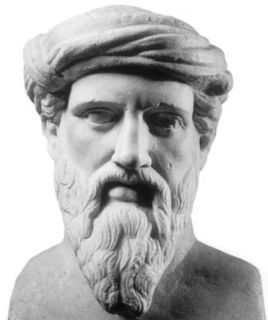
\includegraphics[scale=0.4]{img/Pythagoras.jpg}
 \captionsetup{labelformat=empty}
 \caption{毕达哥拉斯(约前570——前490)}
 \label{fig:Pythagoras}
\end{figure}
%\end{wrapfigure}

从数出发研究世间万物的第一人要算是古希腊的数学家和哲学家毕达哥拉斯。他的名字通过著名的勾股定理(在西方叫毕达哥拉斯定理)而家喻户晓。毕达哥拉斯出生于希腊的萨摩斯(Samos)岛,年轻时他曾去米利都(Miletus)向古希腊哲学的奠基人泰勒斯(Thales)学习。在泰勒斯的建议下,毕达哥拉斯前往东方学习数学。他在埃及学习了13年(一说为22年)。后来波斯帝国征服了埃及,他又随军向东到达了巴比伦,向巴比伦人学习数学和天文知识。或许后来他还到达了更远的印度。不论到了哪里,毕达哥拉斯都不断向有学问的人请教,丰富自己的见解。重要的是,他不仅刻苦学习,而且更善于思考。在经过兼收并蓄、汲取各家之长后,毕达哥拉斯形成并完善了自己的思想\cite{HanXueTao16}。

经历了漫长的在外游历后,年近半百的毕达哥拉斯返回了故乡并开始讲学。公元前520年左右,为了摆脱当地的暴政,毕达哥拉斯移居到了意大利南部的克罗顿(Croton)发展。在那里他赢得了人们的信任与景仰并形成了自己的学派。毕达哥拉斯的弟子中还有女性,学派把主要精力都用来研究天文、几何、数论、音乐这四门学科。它们被称为四术(quadrivium),影响了欧洲教育两千多年\cite{StepanovRose15}。四术体现了毕达哥拉斯“万物皆数”的哲学思想:星体的运动与几何对应,而几何又以数为基础,数字还可以衍生出音乐。毕达哥拉斯是首个发现纯八度音(octave)在频率上有数学规律的人。他的弟子说他可以“听见天界的乐音”\footnote{关于毕达哥拉斯的逝世的说法不一。他领导的学派具有很高的声誉和政治影响,引起了敌对派的忌恨。后来受到民主运动的冲击,学派在克罗顿的活动场所遭到破坏。有人认为毕达哥拉斯被暴徒杀害,也有人说他逃到梅塔蓬图姆(Metapontum)并度过余生。}。

\index{形数(figurate number)}
毕达哥拉斯学派深入研究了数与数、数与自然之间的关系。这开启了数学的重要分支——数论。他们对正整数进行了分类,定义了奇数、偶数、素数、合数等。他们发现某些数的所有真因子\footnote{真因子是小于数本身的因子}之和恰好等于这个数本身,于是将其命名为完全数,并成功地找到两个\footnote{一说为完美数。经过欧几里得与欧拉的进一步工作,揭示了偶完全数的特征以及完全数和梅森素数的关系。到2018年,人们借助计算机发现了前50个梅森素数和完全数。}。最小的完全数是6,因为6 = 1 + 2 + 3,下一个是28(等于1 + 2 + 4 + 7 + 14)。毕达哥拉斯学派还发现了一大类“形数”(figurate number)\footnote{毕达哥拉斯学派的门徒通过在地上摆小石子来研究数字,英文的计算calculus一词就是从希腊文“石子”衍生出的\cite{HanXueTao16}。当他们把石子按照某种几何方式排列成图形时,就得到了形数。}。

\begin{figure}[htbp]
%\begin{wrapfigure}{R}{0.4\textwidth}
\centering
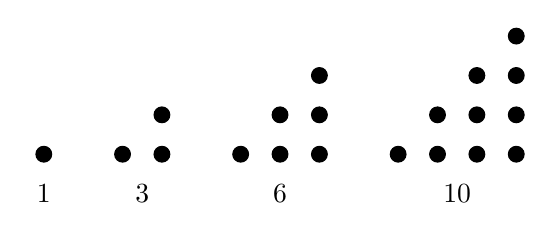
\begin{tikzpicture}[scale=0.5]
\filldraw (0, 0) circle (0.2);
\draw (0, -1) node{1};
\filldraw (2, 0) circle (0.2)
          (3, 0) circle (0.2)   (3, 1) circle (0.2);
\draw (2.5, -1) node{3};
\filldraw (5, 0) circle (0.2)
          (6, 0) circle (0.2)   (6, 1) circle (0.2)
          (7, 0) circle (0.2)   (7, 1) circle (0.2)   (7, 2) circle (0.2);
\draw (6, -1) node{6};
\filldraw (9, 0) circle (0.2)
          (10, 0) circle (0.2)    (10, 1) circle (0.2)
          (11, 0) circle (0.2)    (11, 1) circle (0.2)    (11, 2) circle (0.2)
          (12, 0) circle (0.2)    (12, 1) circle (0.2)    (12, 2) circle (0.2)    (12, 3) circle (0.2);
\draw (10.5, -1) node{10};
\end{tikzpicture}
\caption{三角形数(triangular number)}
\label{fig:triangular-num}
%\end{wrapfigure}
\end{figure}

\begin{figure}[htbp]
%\begin{wrapfigure}{R}{0.4\textwidth}
\centering
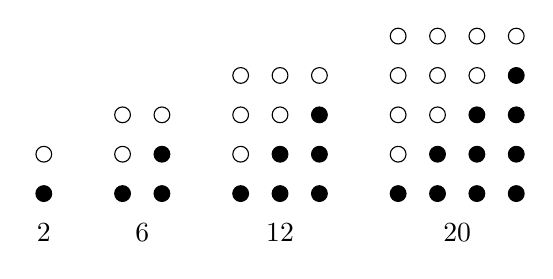
\begin{tikzpicture}[scale=0.5]
\draw (0, 1) circle (0.2);
\filldraw (0, 0) circle (0.2);
\draw (0, -1) node{2};

\draw (2, 1) circle (0.2)   (2, 2) circle (0.2)
      (3, 2) circle (0.2);
\filldraw (2, 0) circle (0.2)
          (3, 0) circle (0.2)   (3, 1) circle (0.2);
\draw (2.5, -1) node{6};

\draw (5, 1) circle (0.2)   (5, 2) circle (0.2)   (5, 3) circle (0.2)
      (6, 2) circle (0.2)   (6, 3) circle (0.2)
      (7, 3) circle (0.2);
\filldraw (5, 0) circle (0.2)
          (6, 0) circle (0.2)   (6, 1) circle (0.2)
          (7, 0) circle (0.2)   (7, 1) circle (0.2)   (7, 2) circle (0.2);
\draw (6, -1) node{12};

\draw (9, 1) circle (0.2)   (9, 2) circle (0.2)   (9, 3) circle (0.2)   (9, 4) circle (0.2)
      (10, 2) circle (0.2)   (10, 3) circle (0.2)   (10, 4) circle (0.2)
      (11, 3) circle (0.2)   (11, 4) circle (0.2)
      (12, 4) circle (0.2);
\filldraw (9, 0) circle (0.2)
          (10, 0) circle (0.2)    (10, 1) circle (0.2)
          (11, 0) circle (0.2)    (11, 1) circle (0.2)    (11, 2) circle (0.2)
          (12, 0) circle (0.2)    (12, 1) circle (0.2)    (12, 2) circle (0.2)    (12, 3) circle (0.2);
\draw (10.5, -1) node{20};
\end{tikzpicture}
\caption{长方形数(oblong number)}
\label{fig:oblong-num}
%\end{wrapfigure}
\end{figure}

图\ref{fig:triangular-num}和图\ref{fig:oblong-num}分别是三角形数和长方形数。很容易看出,每个长方形数都对应三角形数的二倍,而三角形数又是前$n$个正整数之和,这样就得到了正整数累加的求和公式:

\[
1 + 2 + 3 + ... + n = \frac{1}{2}n(n+1)
\]

毕达哥拉斯学派还观察到,所有的奇数可以表示成折尺形(数学上称为“磬折形”)\footnote{gnomon这个字在巴比伦人的原意可能是指日晷上的直杆,用它的阴影来指示时刻。在毕达哥拉斯时代,gnomon指木匠用的方尺。它还表示从正方形的一角切掉一个小正方形后剩余的图形。以后欧几里得又把正方形扩展到平行四边形(\cite{MKlein1972}第一册26页)。},如图\ref{fig:gnomon-num},而前$n$个折尺形可以拼成一个正方形,如图\ref{fig:square-num}。这样他们就发现了前$n$个正奇数的求和公式:

\[
1 + 3 + 5 + ... + (2n - 1) = n^2
\]

\begin{figure}[htbp]
%\begin{wrapfigure}{R}{0.4\textwidth}
\centering
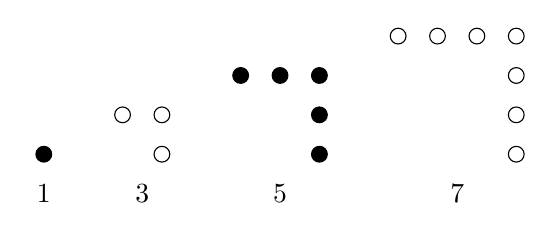
\begin{tikzpicture}[scale=0.5]
\filldraw (0, 0) circle (0.2);
\draw (0, -1) node{1};

\draw (2, 1) circle (0.2)
      (3, 0) circle (0.2)   (3, 1) circle (0.2);
\draw (2.5, -1) node{3};

\filldraw (5, 2) circle (0.2)   (6, 2) circle (0.2)   (7, 2) circle (0.2)
          (7, 0) circle (0.2)   (7, 1) circle (0.2);
\draw (6, -1) node{5};

\draw (9, 3) circle (0.2)   (10, 3) circle (0.2)   (11, 3) circle (0.2)   (12, 3) circle (0.2)
      (12, 0) circle (0.2)    (12, 1) circle (0.2)    (12, 2) circle (0.2);
\draw (10.5, -1) node{7};
\end{tikzpicture}
\caption{折尺形数(gnomon number)}
\label{fig:gnomon-num}
%\end{wrapfigure}
\end{figure}

\begin{figure}[htbp]
%\begin{wrapfigure}{R}{0.4\textwidth}
\centering
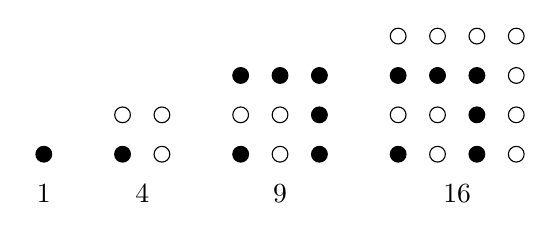
\begin{tikzpicture}[scale=0.5]
\filldraw (0, 0) circle (0.2);
\draw (0, -1) node{1};

\filldraw (2, 0) circle (0.2);
\draw (2, 1) circle (0.2)
      (3, 0) circle (0.2)   (3, 1) circle (0.2);
\draw (2.5, -1) node{4};

\filldraw (5, 0) circle (0.2);
\draw (5, 1) circle (0.2)
      (6, 0) circle (0.2)   (6, 1) circle (0.2);
\filldraw (5, 2) circle (0.2)   (6, 2) circle (0.2)   (7, 2) circle (0.2)
          (7, 0) circle (0.2)   (7, 1) circle (0.2);
\draw (6, -1) node{9};

\filldraw (9, 0) circle (0.2);
\draw (9, 1) circle (0.2)
      (10, 0) circle (0.2)   (10, 1) circle (0.2);
\filldraw (9, 2) circle (0.2)   (10, 2) circle (0.2)   (11, 2) circle (0.2)
          (11, 0) circle (0.2)   (11, 1) circle (0.2);
\draw (9, 3) circle (0.2)   (10, 3) circle (0.2)   (11, 3) circle (0.2)   (12, 3) circle (0.2)
      (12, 0) circle (0.2)    (12, 1) circle (0.2)    (12, 2) circle (0.2);
\draw (10.5, -1) node{16};
\end{tikzpicture}
\caption{正方形数(square number)与折尺形数的关系}
\label{fig:square-num}
%\end{wrapfigure}
\end{figure}

这正是第一章提出的那个习题的答案。就这样,毕达哥拉斯学派发现,很多事物和现象都可以从数的方面进行说明和解释。例如,具有同样张力的两根弦,当它们的长度为简单的整数比时,奏出的乐声就和谐悦耳。由此毕达哥拉斯发展出了最初的音乐理论。音乐与数似乎毫无关系,但它们之间的这种意外联系给毕达哥拉斯很大影响。他从中得到启发并大胆推测:所有的事物都可以用整数或整数的比来解释。毕达哥拉斯学派开始热衷与用数去解释更多的现象,他们相信宇宙的本质就在于“数的和谐”,并且提出“万物皆数”的论断。由此出发,毕达哥拉斯学派试图发展一套以数字为基础的理论,使得几何学可以建立在该理论之上。这种想法实际上就相当于要创建一套基于正整数的统一数学理论。

\index{毕达哥拉斯定理} \index{勾股定理}
毕达哥拉斯学派最著名的发现当属勾股定理的证明。至今这一定理在西方仍被称为“毕达哥拉斯定理”。然而,我们将看到勾股定理是一把双刃剑,他的结果最终形成了一个递归的怪圈,使得“万物皆数”的理念出现了漏洞。为此,我们先要引出可公度概念和欧几里得算法。为了将几何纳入“万物皆数”的理论,毕达哥拉斯学派提出了一个概念来定义一条线段可以用另一条线段来度量。这个定义说,如果一条线段A可以通过有限个另一条线段V来表示时,称线段V可用作线段A的量度(measure)。这本质上是说,我们可以通过整数次拼接产生另一条线段。尽管度量两条不同的线段时,可以使用各自的量度,但是如果想用同一量度测量不同的线段,它必须是二者的公度(common measure)。即当且仅当线段V可以同时成为线段A和线段B的量度时,它才能成为二者的公度。毕达哥拉斯学派认为,任何情况下都可以找到公度,这样几何就可以建立在整数之上了。

%\begin{wrapfigure}{R}{0.4\textwidth}
\begin{figure}[htbp]
 \centering
 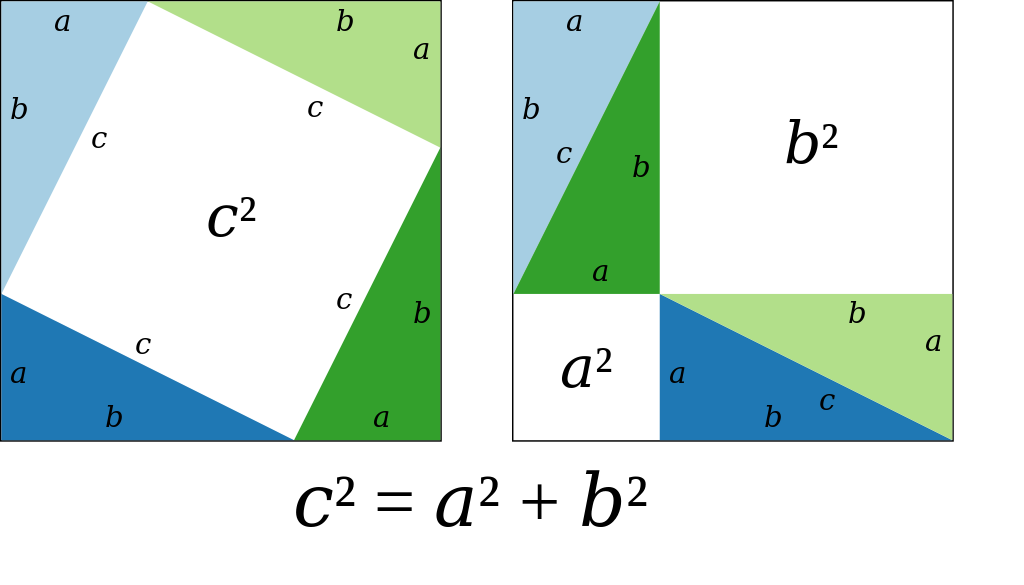
\includegraphics[scale=0.2]{img/Pythagoras-proof.png}
 \caption{勾股定理的一种几何证明,两幅图中白色面积相等(来自《周髀算经》,约公元前200年)}
 \label{fig:Pythagoras-proof}
\end{figure}
%\end{wrapfigure}

\section{欧几里得算法}
\index{最大公度}

由于公度可能有多个,为此需要引入最大公度(greatest common measure)的概念。如果线段V是线段A和线段B的公度,并且比其它公度都大,则称V是A和B的最大公度。已知两条线段,怎样才能求得最大公度呢?这就引出了历史上著名的递归算法——欧几里得算法(又称辗转相除法)。它用古希腊伟大的数学家欧几里得的名字命名\footnote{印度和中国分别独立发现了欧几里得算法。五世纪末,印度数学家阿耶波多(Aryabhata)用这一算法解不定方程(丢番图方程)。在《孙子算经》中,欧几里得算法可以作为中国剩余定理的特例。在1247年,南宋数学家秦九韶在《数书九章》中详细给出了欧几里得算法。}。在欧几里得的名著《几何原本》第十卷命题三中\cite{Elements},详细阐述了这一算法\footnote{在《几何原本》卷七的命题一中,有针对整数的欧几里得算法。但针对线段的情形实际上覆盖了整数。}。

\subsection{欧几里得和《几何原本》}

\begin{wrapfigure}{R}{0.4\textwidth}
%\begin{figure}[htbp]
 \centering
 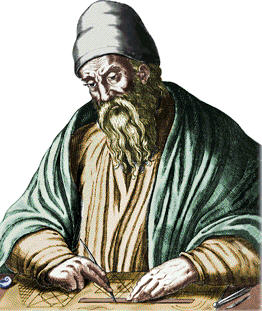
\includegraphics[scale=0.6]{img/Euclid.jpg}
 \captionsetup{labelformat=empty}
 \caption{欧几里得,约公元前300年前后}
 \label{fig:Euclid}
%\end{figure}
\end{wrapfigure}

\index{欧几里得}
欧几里得(Euclid)是古希腊数学家,以其所著的《几何原本》闻名于世。对于他的生平,现在知道的很少。柏拉图学派晚期的导师普罗克洛斯(Proclus)在《几何学发展概要》中记述了这样的趣事:当时的埃及国王,亚历山大的托勒密一世有一次问欧几里得,学习几何学又没有什么捷径可走。欧几里得回答到:“在几何里,没有专为国王铺设的大道。”(There is no royal road to geometry)这句话成为千古传颂的学习箴言\footnote{也译为“几何无王者之道”}。斯托比亚斯(Stobaeus)记述另一则故事说。一个学生刚开始学习第一个命题,就问欧几里得学习几何后将得到什么。欧几里得说:“给他三个钱币,因为他想在学习中获取实利。”由此可知欧几里得主张学习必须循序渐进、刻苦钻研、不赞成投机取巧的作风,也反对狭隘的实用观点(\cite{Elements}中文版序)。

欧几里得的《几何原本》是一部划时代的著作。其伟大的历史意义在于它是用公理建立起演绎体系的最早典范。过去所积累下来的数学知识是零碎的、片断的,可以比作木石砖瓦。只有借助于逻辑方法,把这些知识组织起来,加以分类比较,解释彼此间的内在联系,整理在一个严密的系统之中,才能建成巍峨的大厦。《几何原本》完成了这一艰巨的任务,它对整个数学的发展产生了深远的影响。

两千多年来,这部著作在几何教学中一直占据统治地位,在二十世纪初依然用于数学课的基本教材。包括我国在内的许多国家仍将其作为中学的必修科目(现在中学的几何课本是按照法国数学家拉格朗日《几何原本》改写本思路编写的),并作为训练逻辑推理的最有力教育手段\cite{HanXueTao16}。

\subsection{欧几里得算法}
\index{欧几里得算法}

\begin{proposition}[《几何原本》,卷十,命题三]
已知两个可公度的量,求它们的最大公度量。
\end{proposition}

欧几里得给出的方法,只需要使用递归和减法。因此本质上可以用尺规作图的方式求出最大公度。这一算法可以形式化如下\footnote{名称gcm是最大公度(greatest common measure)的简称。当$a$、$b$是整数时,通常用gcd(greatest common divisor)作为名称。本书按此约定使用这两个名称。}。

\be
gcm(a, b) = \left \{
  \begin{array}
  {r@{\quad:\quad}l}
  a = b & a \\
  b < a & gcm(a - b, b) \\
  a < b & gcm(a, b - a)
  \end{array}
\right.
\label{eq:gcm-minus}
\ee

设两条线段$a$、$b$可公度,如果它们相等,则最大公度就是其中的任一条线段,此时算法返回$a$作为结果。如果线段$a$比$b$长,就用圆规不断从$a$中截去$b$(通过递归),然后求截短的线段$a'$和$b$的最大公度;否则如果线段$b$比$a$长,就反过来不断从$b$中截去$a$,然后求$a$和截短的线段$b'$的最大公度。图\ref{fig:line-seg-gcm}描述了这一算法作用于两条线段的计算步骤。我们也可将这一算法应用于整数42和30并与处理线段的过程进行对比,如下表:

\begin{figure}[htbp]
\centering
\begin{tikzpicture}[scale=0.15]

\filldraw (0, 0) circle (0.5)   (30, 0) circle (0.5)   (42, 0) circle (0.5);
\draw (-8, 0) node{$a$} (0, 0) -- (42, 0);
\filldraw (0, -5) circle (0.5)   (30, -5) circle (0.5);
\draw (-8, -5) node{$b$} (0, -5) -- (30, -5);

\filldraw (0,  -15) circle (0.5)   (12, -15) circle (0.5);
\draw (-8, -15) node{$a'=a-b$} (0, -15) -- (12, -15);
\filldraw (0, -20) circle (0.5)   (12, -20) circle (0.5)   (24, -20) circle (0.5)   (30, -20) circle (0.5);
\draw (-8, -20) node{$b$} (0, -20) -- (30, -20);

\filldraw (0,  -30) circle (0.5)   (6, -30) circle (0.5)   (12, -30) circle (0.5);
\draw (-8, -30) node{$a'$} (0, -30) -- (12, -30);
\filldraw (0, -35) circle (0.5)   (6, -35) circle (0.5);
\draw (-8, -35) node{$b'=b-2a'$} (0, -35) -- (6, -35);

\filldraw (0,  -45) circle (0.5)   (6, -45) circle (0.5);
\draw (-8, -45) node{$a''=a'-b'$} (0, -45) -- (6, -45);
\filldraw (0, -50) circle (0.5)   (6, -50) circle (0.5);
\draw (-8, -50) node{$b'$} (0, -50) -- (6, -50);

\end{tikzpicture}
\caption{欧几里得算法的线段示意}
\label{fig:line-seg-gcm}
\end{figure}

\begin{tabular}{|l|l|l|}
\hline
$gcm(a, b)$ & $a$ & $b$ \\
\hline
$gcm(42, 30)$ & 42 & 30 \\
\hline
$gcm(12, 30)$ & 12 & 30 \\
\hline
$gcm(12, 18)$ & 12 & 18 \\
\hline
$gcm(12, 6)$ & 12 & 6 \\
\hline
$gcm(6, 6)$ & 6 & 6 \\
\hline
\end{tabular}
\vspace{5mm}

将一个量$b$反复从另一个量$a$中减去,最后得到$a'$的过程恰好是带余数除法的定义。即$a' = a - \lfloor a / b \rfloor b$或记为$a'= a \bmod b$。因此我们可以用除法和求余运算代替原始欧几里得算法中的反复相减。此外,当一个量是另一个量的整倍数时,例如$b \leq a$且$b$可以整除$a$,我们立即知道最大公度为$b$。此时求余的结果$a \bmod b = 0$,为此我们可以定义$gcm(0, b) = gcm(b, 0) = b$。我们可以先比较$a$和$b$的大小,如果$a < b$就交换两个量。由于我们知道$a \bmod b$一定小于$b$, 所以下次递归时可以直接交换为:$gcm(b, a \bmod b)$。这样就得到了改进的欧几里得算法。

\be
gcm(a, b) = \left \{
  \begin{array}
  {r@{\quad:\quad}l}
  b = 0 & a\\
  \text{否则} & gcm(b, a \bmod b) \\
  \end{array}
\right.
\label{eq:gcm}
\ee

为什么这个算法可以求出最大公度呢?我们需要分两步来证明它的正确性。第一步我们要证明这一算法可以求出公度。设$b \leq a$,令整数$q_0$为商,$r_0$为余数,即$a = b q_0 + r_0$,如果$r_0$为零,算法就找到了公度,为此我们考虑$r_0$不为零的情况。此时可以进一步列出$b = r_0 q_1 + r_1$,类似地,只要余数不为零,我们可以一直列出这样的式子。

\[
\begin{array}{rcl}
a &=& b q_0 + r_0 \\
b &=& r_0 q_1 + r_1 \\
r_0 &=& r_1 q_2 + r_2 \\
r_1 &=& r_2 q_3 + r_3 \\
& & ...
\end{array}
\]

但只要$a$、$b$是可公度的,这些式子不会无限列下去。理由是每次都用圆规截取整数次,即商是整数。同时每次都保证余数小于除数。即$b > r_0 > r_1 > r_2 > ... > 0$,但是余数不可能小于零。由于起始值是有限的,故最终一定在有限步内得到$r_{n-2} = r_{n-1} q_n$。

接下来我们证明最后一步得到的$r_{n-1}$可以同时度量$a$和$b$。根据度量的定义,显然$r_{n-1}$可以度量$r_{n-2}$。然后考虑倒数第二式$r_{n-3} = r_{n-2} q_{n-1} + r_{n-1}$,由于$r_{n-1}$可以度量$r_{n-2}$,所以$r_{n-1}$也可以度量$r_{n-2} q_{n-1}$,自然它也可以度量$r_{n-2} q_{n-1} + r_{n-1}$,这个量恰好等于$r_{n-3}$。用同样的方法,我们可以向上逐一证明$r_{n-1}$可以度量每个式子左边,一直到$b$、$a$。这样我们就证明了欧几里得算法得到的答案$r_{n-1}$是$a$、$b$的公度。若最大公度为$g$,一定有$r_{n-1} \leq g$。

第二步我们要证明,任何$a$、$b$的公度$c$,一定也可以度量$r_{n-1}$。由于$c$是公度,因此$a$和$b$可以用它来表示,不妨记$a = mc$、$b = nc$,其中$m$、$n$都是整数。这样第一式$a = b q_0 + r_0$就可以写成$mc = ncq_0 + r_0$,我们得知$r_0 = (m - nq_0)c$,因此$c$也可以度量$r_0$。类似地,我们可以依次证明$c$可以度量$r_1$、$r_2$、……、$r_{n-1}$。这样我们就证明了任何公度都可以度量$r_{n-1}$,因此最大公度$g$也可以度量$r_{n-1}$,即$g \leq r_{n-1}$。

综合第一、二步的结果,即$r_{n-1} \leq g$且$g \leq r_{n-1}$,我们得出最大公度$g = r_{n-1}$,也就是说欧几里得算法能够正确地给出最大公度。进一步,我们知道$g$是每一对量的最大公度,即:

\be
g = gcm(a, b) = gcm(b, r_0) = ... = gcm(r_{n-2}, r_{n-1}) = r_{n-1}
\label{eq:recursive-gcm}
\ee

\begin{figure}[htbp]
 \centering
 \subcaptionbox{反复剪掉正方形}{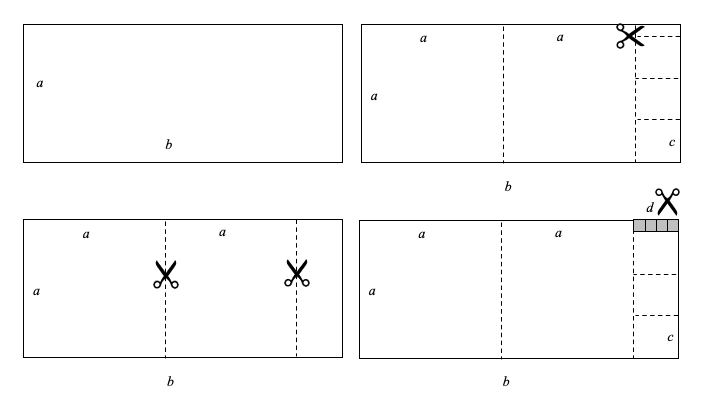
\includegraphics[scale=0.45]{img/GCM.png}}
 \subcaptionbox{用最终的小正方形铺满原图}{
   \begin{adjustbox}{max width=\textwidth}
   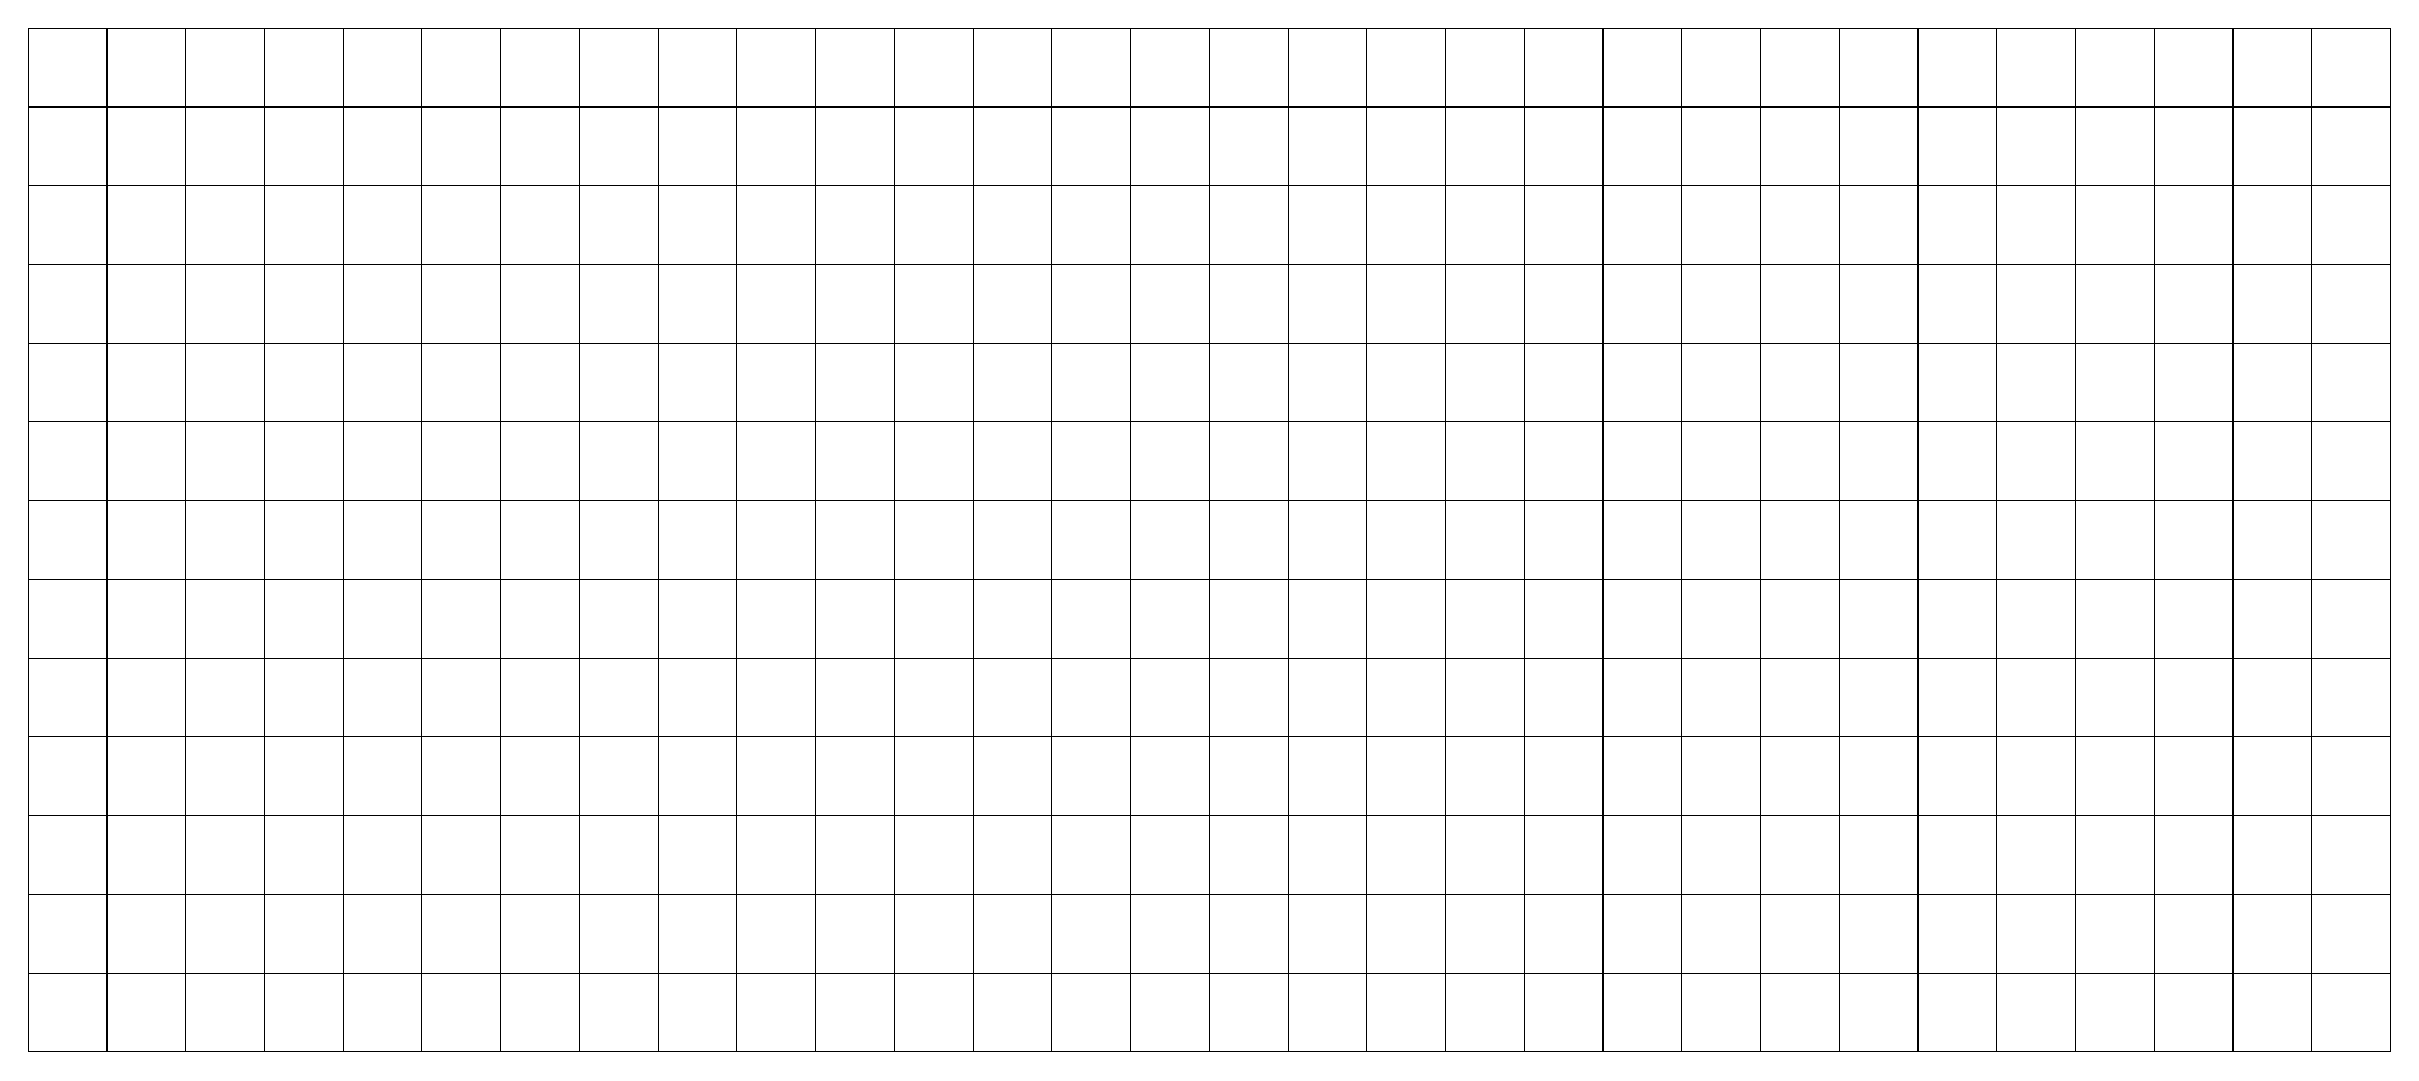
\begin{tikzpicture}
     \draw[step=1, thin] (0, 0) grid (30, 13);
   \end{tikzpicture}
   \end{adjustbox}
 }
 \captionsetup{labelformat=empty}
 \caption{欧几里得算法的几何解释}
 \label{fig:geometric-GCM}
\end{figure}

\subsection{扩展欧几里得算法}

\index{扩展欧几里得算法} \index{贝祖等式}
所谓扩展欧几里得算法,就是除了求得两个量$a$、$b$的最大公度$g$外,同时找到满足贝祖等式$ax + by = g$的两个整数$x$和$y$。为什么贝祖等式(Bézout's identity)\footnote{贝祖等式,或称贝祖定理(也译为裴蜀定理),最早是由法国数学家梅齐里亚克(Claude Gaspard Bachet de Méziriac,1581–1638)发现并证明了其对整数成立,法国数学家贝祖证明这一等式对多项式成立。贝祖等式可以推广到任意的整环和主理想环(PID,Principle Ideal Domain)上。}一定成立呢?我们下面给出贝祖等式的一种证明。由$a$、$b$可以构造一个集合,包含它们所有正的线性组合:

\[
S = \{ ax + by | x, y \in \mathbb{Z} \text{且} ax + by > 0\}
\]

%\begin{wrapfigure}{R}{0.4\textwidth}
\begin{figure}[htbp]
 \centering
 \subcaptionbox{贝祖(Étienne Bézout, 1730 - 1783)}[0.45\linewidth]{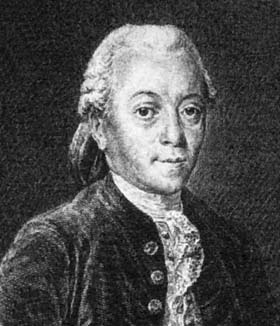
\includegraphics[scale=0.45]{img/Bezout.jpeg}}
 \subcaptionbox{梅齐里亚克(Claude Gaspard Bachet de Méziriac, 1581–1638),最早发现并证明了整数上的贝祖等式。}[0.45\linewidth]{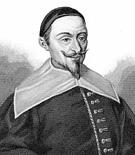
\includegraphics[scale=0.95]{img/Meziriac.jpg}}
 \captionsetup{labelformat=empty}
 \caption{}
 \label{fig:Bezout}
 \label{fig:Meziriac}
\end{figure}
%\end{wrapfigure}

对于线段来说,$S$一定不为空,因为它至少包含$a$(此时$x = 1, y = 0$)和$b$(此时$x = 0, y = 1$)。因为$S$的所有元素都为正,所以它一定存在一个最小的元素,我们将其记为$g = as + bt$。我们接下来要证明$g$就是$a$和$b$的最大公度。为此我们将$a$表示成$g$的商与余数的形式。

\be
a = qg + r
\label{eq:Euclidean-division}
\ee

其中余数$0 \leq r < g$。余数要么为0,要么在集合$S$中。这是因为

\[
\begin{array}{rll}
r & = a - qg & \text{由式(\ref{eq:Euclidean-division})} \\
  & = a - q(as + bt) & g\text{的定义} \\
  & = a(1 - qs) - bqt & \text{合并整理}
\end{array}
\]

即$r$可以表示为$a$、$b$的线性组合,因此如果它不为0,则一定在集合$S$中。但这是不可能的,因为我们之前假设$g$是$S$中的最小正元素,而$r$却比$g$更小,这样就会产生矛盾。因此我们的得知$r$一定等于0。根据式(\ref{eq:Euclidean-division}),$g$一定可以度量$a$。用同样的方法,可以证明$g$也一定可以度量$b$。因此$g$是它们的公度。接下来我们证明$g$是最大公度。令$c$为$a$和$b$的任意公度,根据定义,存在整数$m$、$n$使得$a = mc$、$b = nc$。这样$g$就可以表示为:

\[
\begin{array}{rll}
g & = as + bt & \text{由定义} \\
  & = mcs + nct & c\text{是$a$、$b$的公度} \\
  & = c(ms + nt) & g\text{是$c$的倍数}
\end{array}
\]

这说明$c$可以度量$g$,也就是说$c \leq g$。这就证明了$g$是最大公度。综上我们就证明了贝祖等式,即存在整数使得$ax + by = g$,并且进一步得知最大公度是所有线性组合的正值中最小的。

使用贝祖等式,我们可以推导出扩展欧几里得算法。

\[
\begin{array}{rlr}
ax + by & = gcm(a, b) & \text{贝祖等式} \\
        & = gcm(b, r_0) & \text{欧几里得算法,式(\ref{eq:recursive-gcm})} \\
        & = bx' + r_0 y' & \text{对$b$和$r_0$使用贝祖等式} \\
        & = bx' + (a - bq_0)y' & \text{利用$a = b q_0 + r_0$} \\
        & = ay' + b(x' - y'q_0) & \text{整理为$a$和$b$的线性组合} \\
        & = ay' + b(x' - y' \lfloor a / b \rfloor) & \text{将$q_0$表示为$a$与$b$的商}
\end{array}
\]

这样就得出了每次递归时的关系:

\[
\left \{
  \begin{array}{l}
  x = y' \\
  y = x' - y' \lfloor a / b \rfloor
  \end{array}
\right.
\]

递归的边界条件出现在$b = 0$的时候,此时$gcm(a, 0) = 1a + 0b$。把边界条件和递归关系归纳起来就得到了扩展欧几里得算法。

\be
gcm_{ex}(a, b) = \left \{
  \begin{array}
  {r@{\quad:\quad}l}
  b = 0 & (a, 1, 0) \\
  \text{否则} & \begin{array}{l}
                (g, y', x' - y' \lfloor a / b \rfloor) \\[2pt]
                \text{其中}(g, x', y') = gcm_{ex}(b, a \bmod b)
                \end{array} \\
  \end{array}
\right.
\label{eq:gcm-ext}
\ee

我们下面给出一个使用扩展欧几里得算法解决的趣题(\cite{LiuXinyu2017},第450页)。有两个水瓶,一个的容量是9升,另一个的容量是4升。问如何才能从河中打出6升水?

这道题目有很多变化形式,瓶子的容积和取水的容量可以是其它数值。有一个故事说解决这道题目的主人公是少年时代的法国数学家泊松(Sim\`{e}on Denis Poisson)。

使用两个瓶子,共有6种操作。记大瓶子为$A$,容积为$a$;小瓶子为$B$,容积为$b$:

\begin{itemize}
\item 将大瓶子$A$装满水;
\item 将小瓶子$B$装满水;
\item 将大瓶子$A$中的水倒空;
\item 将小瓶子$B$中的水倒空;
\item 将大瓶子$A$中的水倒入小瓶子$B$;
\item 将小瓶子$B$中的水倒入大瓶子$A$。
\end{itemize}

其中最后两种操作中,任意一个瓶子满或者另一个瓶子空时就停止。表\ref{tab:jug-ops}给出了一系列倒水动作的例子,这里假设容积$b < a < 2b$。

\begin{table}[htbp]
\centering
\begin{tabular}{l|l|l}
$A$ & $B$ & 操作 \\
\hline
0 & 0 & 开始 \\
0 & b & 倒满$B$ \\
b & 0 & 将$B$倒入$A$ \\
b & b & 倒满$B$ \\
a & 2b - a & 将$B$倒入$A$ \\
0 & 2b - a & 倒光$A$ \\
2b - a & 0 & 将$B$倒入$A$ \\
2b - a & b & 倒满$B$ \\
a & 3b - 2a & 将$B$倒入$A$ \\
... & ... & ... \\
\end{tabular}
\caption{两个瓶子内的水量和倒水操作的对应关系} \label{tab:jug-ops}
\end{table}

无论进行何种操作,每个瓶子中的水的容量总可以表示为$ax + by$的形式,其中$x$、$y$是整数。也就是说,我们能获得的水的体积总是$a$与$b$的线性组合。根据贝祖等式的证明,我们知道线性组合的最小正值恰好是$a$和$b$的最大公度$g$。
因此给定两个瓶子的容量,我们立即能够判断是否可以得到体积为$c$的水——只要$c$能够被$g$度量\footnote{如果容积为整数,当且仅当$c$能够被最大公约数$g$整除。}。当然还要求$c$不能超过两个瓶子中较大瓶子的容积。

例如,使用容量为4升和6升的瓶子,我们永远无法得到5升水。这是因为4与6的最大公约数是2,但5不能被2整除。(换个思路想这个问题:用两个容积为偶数升的瓶子,永远无法从河里打到奇数升的水。)如果$a$和$b$是互素的整数,即$gcd(a, b) = 1$,则可以得到任意自然数$c$升的水。

虽然通过检查$g$是否能度量$c$可以判断是否有解,但是我们并不知道具体的倒水步骤。如果我们可以找到整数$x$和$y$,使得$ax + by = c$。就可以得到一组操作来解决此题。具体思路是这样的:若$x > 0$、$y < 0$,我们需要倒满瓶子$A$共$x$次,倒空瓶子$B$共$y$次;反之若$x < 0$、$y > 0$,则需要倒空瓶子$A$共$x$次,倒空瓶子$B$共$y$次。

例如,若大瓶容积$a=5$、小瓶容积$b=3$,要取得$c=4$升水,因为$4 = 3 \times 3 - 5$,即$x = -1$、$y = 3$我们可以设计下表中的一系列操作。

\begin{table}[htbp]
\centering
\begin{tabular}{l|l|l}
$A$ & $B$ & 操作 \\
\hline
0 & 0 & 开始 \\
0 & 3 & 倒满$B$ \\
3 & 0 & 将$B$倒入$A$ \\
3 & 3 & 倒满$B$ \\
5 & 1 & 将$B$倒入$A$ \\
0 & 1 & 将$A$倒空 \\
1 & 0 & 将$B$倒入$A$ \\
1 & 3 & 倒满$B$ \\
4 & 0 & 将$B$倒入$A$ \\
\end{tabular}
\caption{取得4升水需要进行的操作} \label{tab:designed-jugs-ops}
\end{table}

在这一系列操作中,倒满$B$共3次,倒空$A$共1次。因此剩下的问题是如何寻找整数$x$和$y$。使得$ax + by = c$,根据扩展欧几里得算法,我们可以找到满足贝祖等式的一组解$ax_0 + by_0 = g$。因为$c$是最大公度$g$的$m$倍,我们只要把$x_0$和$y_0$相应加大$m$倍即可得到一组特解:

\[
\begin{dcases}
  x_1 = x_0 \dfrac{c}{g} \\
  y_1 = y_0 \dfrac{c}{g}
\end{dcases}
\]

根据这组特解,我们可以找到满足不定方程\footnote{又叫做丢番图方程,是用古希腊亚历山大的数学家丢番图(Diophantus,约200-284)的名字命名的。丢番图在他的著作《算术》中,独创地引入了代数符号系统。被一些数学史家誉为“代数学之父”\cite{HanXueTao2009}。}的所有整数解:

\be
\begin{dcases}
  x = x_1 - k \dfrac{b}{g} \\
  y = y_1 + k \dfrac{a}{g}
\end{dcases}
\ee

这里$k$为整数。这样我们就找到了倒水问题的所有解。进一步,我们可以找到一个特定的$k$,使得$|x| + |y|$的值最小,从而得到最快的倒水步骤\footnote{例如,可以将表示解的两条直线画出。取绝对值后,将横轴下方的部分对称翻转。进而找到使得$|x|+|y|$最小的$k$。}。下面是解决这一趣题的Haskell例子程序。

\lstset{frame=single}
\begin{lstlisting}
import Data.List
import Data.Function (on)

-- Extended Euclidean Algorithm
gcmex a 0 = (a, 1, 0)
gcmex a b = (g, y', x' - y' * (a `div` b)) where
  (g, x', y') = gcmex b (a `mod` b)

-- Solve the linear Diophantine equation ax + by = c
solve a b c | c `mod` g /= 0 = (0, 0, 0, 0) -- no solution
            | otherwise = (x1, u, y1, v)
  where
    (g, x0, y0) = gcmex a b
    (x1, y1) = (x0 * c `div` g, y0 * c `div` g)
    (u, v) = (b `div` g, a `div` g)

-- Optimal by minimize |x| + |y|
jars a b c = (x, y) where
  (x1, u, y1, v) = solve a b c
  x = x1 - k * u
  y = y1 + k * v
  k = minimumBy (compare `on` (\i -> abs (x1 - i * u) +
                                     abs (y1 + i * v))) [-m..m]
  m = max (abs x1 `div` u) (abs y1 `div` v)
\end{lstlisting}

求得两个瓶子倒空和倒满的次数$x$、$y$后,就可以生成一系列倒水的步骤,本章附录提供了完整的例子程序。

\subsection{欧几里得算法的意义}

在“万物皆数”的哲学思想下,虽然欧几里得算法最初是为了寻找两个整数的最大公约数而产生的。但是经过欧几里得之手,算法却应用到了抽象的几何量上。从整数的最大公约数,到可公度量的最大公度,我们看到了几何量和数的分离\footnote{这也是我们使用gcm,而没有使用更常见的gcd作为算法简写的原因。}。几何不仅没有建立在整数之上,反而独立发展,解决了整数之外的问题。以至于后来古希腊数学形成了这样的传统,任何关于数的结论,都需要给出几何的证明。这一传统直到十六世纪仍然影响着人们。意大利数学家卡尔丹(Gerolamo Cardano)\footnote{也译作卡尔达诺}在关于解三次、四次方程的著作《大术》(Ars Magna,1545年出版)中,仍然使用类似立方体填补法的几何论证\cite{HanXueTao2009}。

欧几里得算法是最著名的一个递归算法。德国数学家,解析数论创始人狄利克雷(Dirichlet)在他的著作《数论讲义》中评价到:“整个数论的结构都建立在同一个基础之上,这个基础就是最大公约数算法。”现代密码学的RSA加密算法\footnote{RSA算法是最早的一种公开密钥加密的非对称加密算法,RSA是1977年由罗纳德·李维斯特(Ron Rivest)、阿迪·萨莫尔(Adi Shamir)和伦纳德·阿德曼(Leonard Adleman)一起提出的。当时他们三人都在麻省理工学院工作。RSA就是他们三人姓氏开头字母拼在一起组成的。}直接使用了扩展欧几里得算法。我们在上一节通过一道趣题展示了如何使用扩展欧几里得算法给出二元线性不定方程$ax + by = c$的整数解。具体来说,就是先求出最大公度$g$,并判断$g$是否整除$c$,若不能,则无整数解。否则,将满足贝祖等式的$x_0$,$y_0$,扩大$c/g$倍得到一组特解$x_1$、$y_1$。然后得到一般二元线性不定的通解$x = x_1 - k b / g$和$y = y_1 + k a / g$。

%\begin{wrapfigure}{R}{0.4\textwidth}
\begin{figure}[htbp]
 \centering
 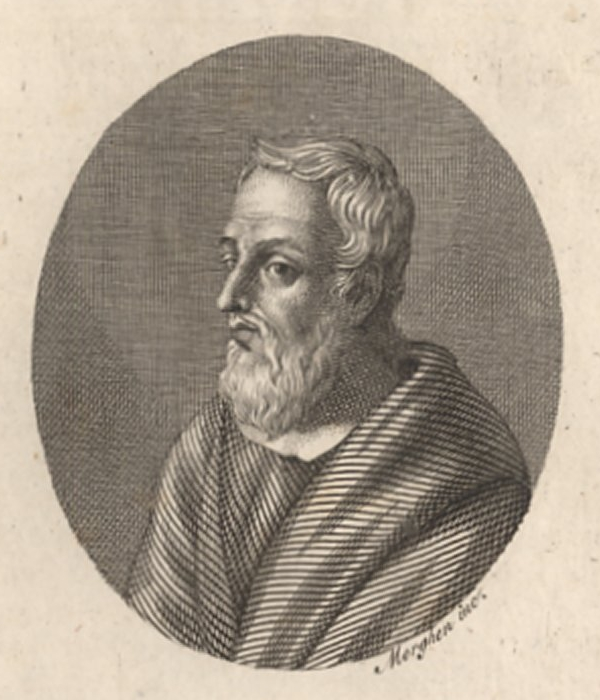
\includegraphics[scale=0.25]{img/Hippasus.jpg}
 \captionsetup{labelformat=empty}
 \caption{希帕索思(Hippasus of Metapontum)约公元前五世纪。}
 \label{fig:Hippasus}
\end{figure}
%\end{wrapfigure}

\index{希帕索思(Hippasus of Metapontum)}
欧几里得算法是一把锋利的宝剑,但是它强大的递归原理被反过来指向了“万物皆数”的基石——万物可公度。一切事物和现象都可以归结为整数与整数的比。从而引发了毕达哥拉斯学派哲学思想的危机。约公元前470年左右,毕达哥拉斯学派的学生希帕索思试图寻找正方形的对角线和边的公度。经过仔细思考他发现不管度量单位取得多么小,这两条线段都无法公度。还有的说法是希帕索思从毕达哥拉斯学派的神秘五角星标志上得到了启发。毕达哥拉斯学派成员用五角星作为学派的徽章和联络标志。有一则故事说,学派的一个成员流落异乡,贫病交迫,无力酬谢房主的款待,临终前要房主在门上画一个五角星。若干年后,有同派的人看到这个标志,询问事情的经过,厚报房主而去\cite{HanXueTao16}。美国迪士尼在1959年的动画片《唐老鸭漫游数学奇境》中,描绘了唐老鸭遇到了毕达哥拉斯和他的朋友们,在了解音乐、艺术与数的关系后,唐老鸭的手掌上也画上了神秘的五角星。如图\ref{fig:pentagram}所示,传说希帕索思发现线段AC和AG也是无法公度的。

%《唐老鸭漫游数学奇境》(Donald In Mathmagic Land )

%\begin{wrapfigure}{L}{0.4\textwidth}
\begin{figure}[htbp]
 \centering
 \subcaptionbox{递归的五角星}[0.45\linewidth]{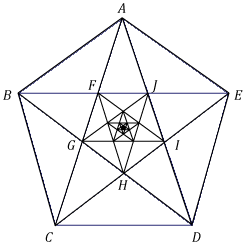
\includegraphics[scale=0.5]{img/pentagram.png}}
 \subcaptionbox{正方形的边长和对角线}[0.45\linewidth]{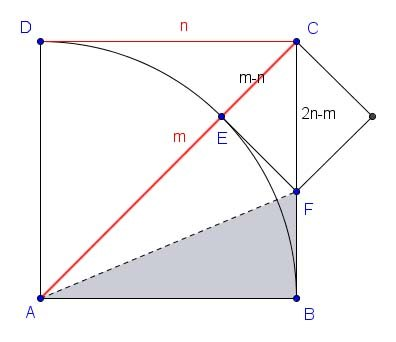
\includegraphics[scale=1.5]{img/irrational.jpg}}
 %\captionsetup{labelformat=empty}
 \caption{}
 \label{fig:pentagram}
 \label{fig:irrational}
\end{figure}
%\end{wrapfigure}

十九世纪的苏格兰数学家乔治$\cdot$克里斯托重建了希帕索思的证明。使用反证法,假设存在一条单位线段$c$能够公度正方形的边和对角线。根据度量的定义,可以令边长为$mc$、对角线长为$nc$,其中$m$、$n$都是正整数。如图\ref{fig:irrational}所示,我们以点A为圆心,以边长为半径做圆弧交对角线AC于点E。然后从E出发作垂直于对角线的直线,并交边BC于点F。

根据圆的定义,线段AE的长度等于正方形的边长,所以线段EC的长度等于$(m - n)c$。因为EF垂直于AC,而角$\angle ECF$是$45\degree$,故三角形ECF是等腰直角三角形。由于等腰三角形两腰相等,故而有$|EC| = |EF|$。接下来我们注意两个直角三角形$\triangle AEF$和$\triangle ABF$,由于边AE等于AB,同时AF是公共边,因此两个直角三角形全等。这样就得到边$|EF| = |FB|$。综合下来,我们有$|EC| = |EF| = |FB|$。这样线段FB的长度也等于$(m - n)c$,所以线段CF的长度等于CB的长度减去FB的长度,等于$nc - (m - n)c = (2n - m)c$。我们把得到的结论列在下面。

\[
\begin{array}{c|c}
\begin{cases}
|AC| = mc \\
|AB| = nc
\end{cases} &
\begin{cases}
|CF| = (2n - m)c \\
|CE| = (m - n)c
\end{cases} \\[4ex]
\text{大正方形} & \text{小正方形}
\end{array}
\]

由于$m$、$n$都是正整数,显然$c$也可以公度小正方形的对角线$CF$和边$CE$。仿照上面的方法,我们可以继续作出更小的正方形,并且重复作出无穷无尽的更小的正方形。而$c$总可以公度每一个小正方形的斜边和对角线。由于$m$、$n$是有限的正整数,这一过程不可能无限做下去,这样就产生了矛盾。于是我们一开始的假设不成立,即正方形的边和对角线不可公度。

这样毕达哥拉斯万物皆数的理论就出现了一个漏洞:存在线段的长度无法用整数比进行度量。据说希帕索思因为这个发现,而遭到谋杀,毕达哥拉斯学派担心这个秘密被泄露出去,而把希帕索思沉入大海。然而历史的车轮不会倒退,古希腊的哲学家和数学家们正视了这个问题,经过欧多克索斯、亚里士多德和欧几里得等人的工作,终于严格定义了不可公度和无理量,并通过几何将它们纳入了古希腊的数学体系。

\index{不可公度}
\begin{proposition}[《几何原本》,卷十,命题二]
如果从两个不等量的大量中连续减去小量,直到余量小于小量,再从小量中连续减去余量直到小于余量,这样一直作下去,当所余的量总不能量尽它前面的量时,则称两个量不可公度。
\end{proposition}

这里出现了一个有趣的现象,不可公度是用欧几里得算法能否停止来定义的。由于欧几里得算法是递归的,也就是说递归能否中止成了判断条件。这再次将我们的注意力引入到递归的本质上。递归究竟是什么?它怎样用形式化的方法表示?

\begin{Exercise}
\Question{我们给出的欧几里得算法是递归的,请消除递归,只使用循环实现欧几里得算法和扩展欧几里得算法。}
\Question{大多数编程环境中的取模运算,要求除数、被除数都是整数。但是线段的长度不一定是整数,请实现一个针对线段的取摸运算。它的效率如何?}
\Question{我们在证明欧几里得算法正确性的过程中说:“每次都保证余数小于除数。即$b > r_0 > r_1 > r_2 > ... > 0$,但是余数不可能小于零。由于起始值是有限的,故最终算法一定中止。”为什么不会出现,$r_{n}$无限接近于零但不等于零的情况?算法一定会中止么?$a$和$b$是可公度的这一前提保证了什么?}
\Question{对于二元线性不定方程$ax + by = c$,若$x_1$、$y_1$和$x_2$、$y_2$为两对整数解。试证明$|x_1 - x_2|$的最小值为$b/gcm(a, b)$,且$|y_1 - y_2|$的最小值为$a/gcm(a, b)$。}
\Question{边长为1的正五边形,对角线的长度是多少?试证明图\ref{fig:pentagram}的五角星中的线段AC和AG是不可公度的。使用实数表示,它们的比值是什么?}
\end{Exercise}

\section{$\lambda$演算}

如果进行计算的是如我们人类这样的智慧生命,也许不用深究递归的原理。我们只需要进行计算,发现递归时就在自己的思维中螺旋进入下一个层次。当递归终止时,就退回上一层。当人们思考如何用机器帮助我们进行计算时,这一问题才变得重要起来。二十世纪三十年代,当人们在研究可计算问题时,分别独立提出了一些计算模型。最著名的包括图灵提出的图灵机模型(1935年),丘奇(1932到1941年)和克莱尼(Stephen Kleene,1935年)提出的$\lambda$演算(希腊字母$\lambda$读作lambda),埃尔布朗(Jacques Herbrand)和哥德尔(Kurt Gödel)提出的递归函数(1934年)等。

%\begin{wrapfigure}{L}{0.35\textwidth}
\begin{figure}[htbp]
 \centering
 \subcaptionbox{艾伦$\cdot$图灵(Alan Mathison Turing,1912 - 1954)}[0.45\linewidth]{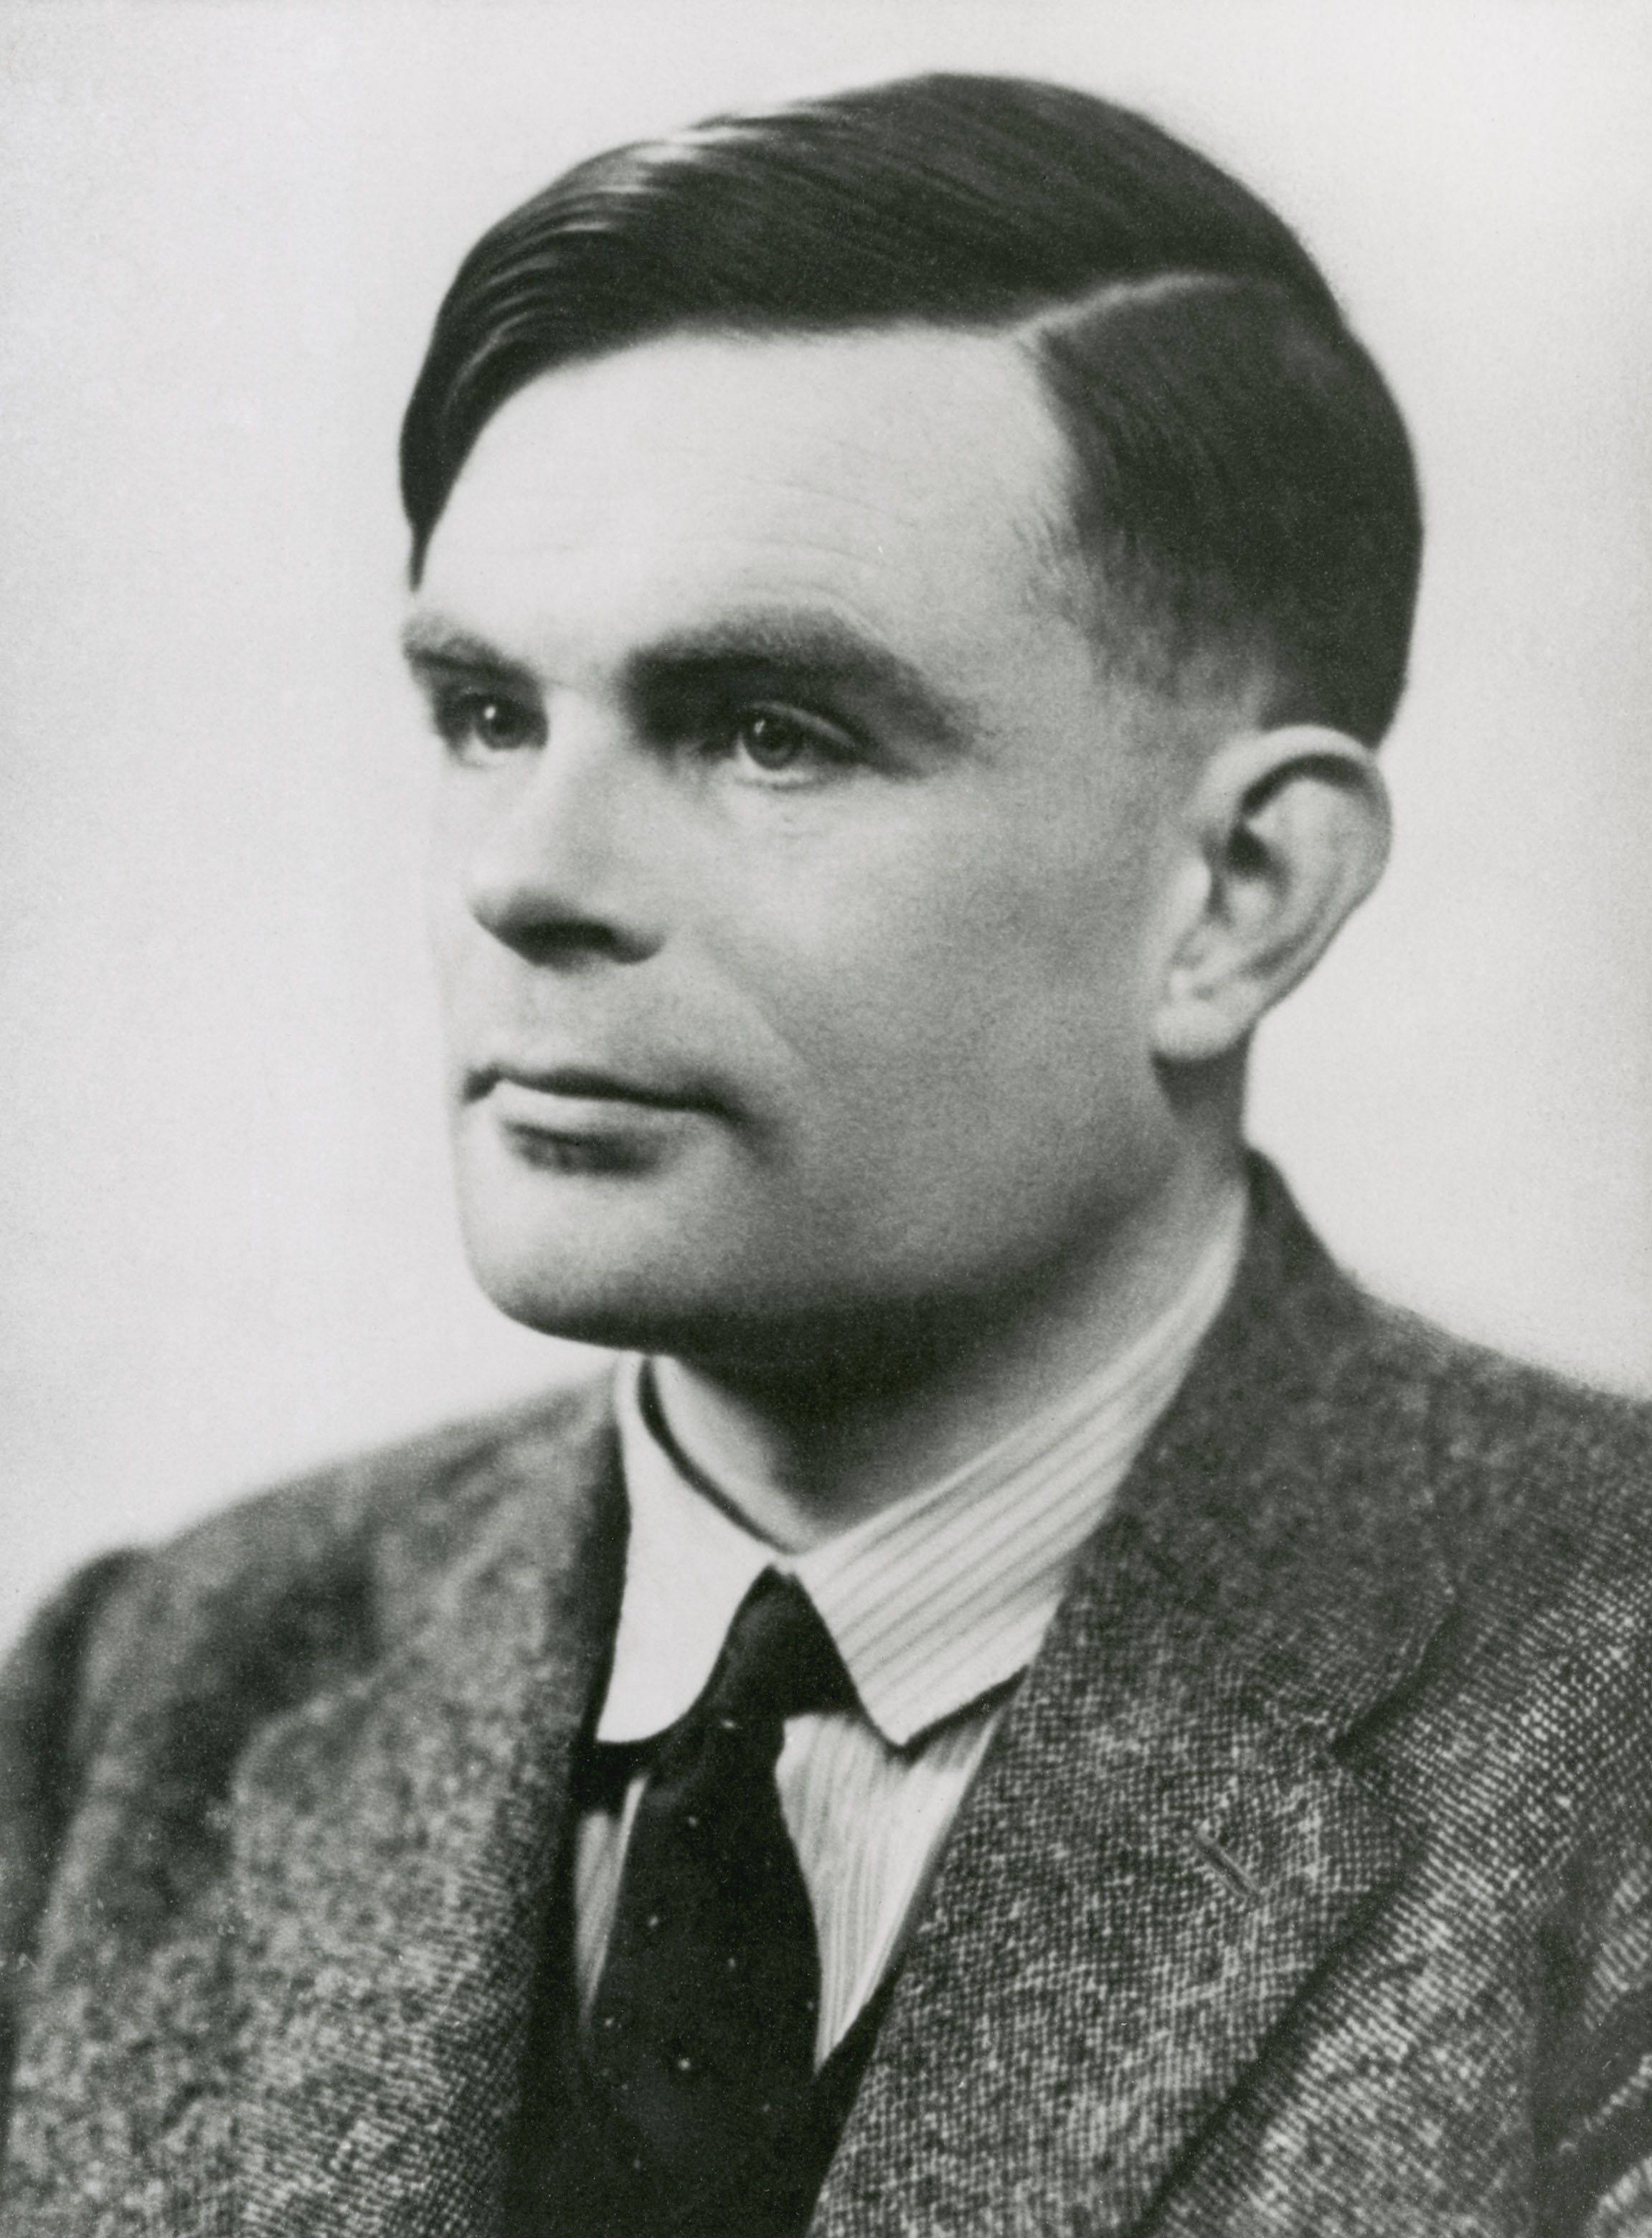
\includegraphics[scale=0.2]{img/Turing.jpg}} \quad
 \subcaptionbox{阿隆佐$\cdot$丘奇(Alonzo Church, 1903 - 1995)}[0.45\linewidth]{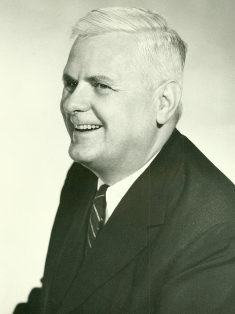
\includegraphics[scale=0.65]{img/Church.jpg}}
 \captionsetup{labelformat=empty}
 \label{fig:Turing}
 \label{fig:Church}
\end{figure}
%\end{wrapfigure}

\index{图灵}
图灵是英国数学家、逻辑学家,深刻地影响了计算机科学的理论发展,他提出使用图灵机来形式化算法和计算的概念,是现代通用计算机的模型。图灵因此被称为计算机科学之父和人工智能之父\cite{wiki-Turing}。第二次世界大战期间,图灵参加了盟军位于布莱切利公园的密码破译中心。他设计了很多技术用以快速破解纳粹德国的密码。图灵研制了一台绰号为“炸弹”(Bombe)的电子机器,使用战前波兰发现的方法,可以在一小时内找到德军恩尼格玛(Enigma)密码机的密钥。密码的成功破译是盟国获胜的一个关键因素,许多历史学家认为缩短了战争达2年之多,并且挽救了成千上万的生命。战争结束后,图灵开始从事“自动计算机”(ACE)的逻辑设计和具体研制工作。在图灵的设计思想指导下,1950年制出了ACE样机,1958年制成大型ACE机。人们认为,通用计算机的概念就是图灵提出来的。1950年,图灵开始考虑机器思维的问题并在论文《计算机与智能》中提出了著名的“图灵测试”。这一划时代的作品,使图灵赢得了“人工智能之父”的桂冠。1951年,由于在可计算数学方面所取得的成就,图灵成为英国皇家学会会员,时年39岁。为了纪念他对计算机科学的巨大贡献,由美国计算机协会(ACM)于1966年设立一年一度的图灵奖,以表彰在计算机科学中做出突出贡献的人,图灵奖被喻为“计算机界的诺贝尔奖”。

\index{lambda演算}
对计算本身进行形式化,被称为“元数学”。这一试图重新为计算树立数学地位的尝试产生了一个杰作——$\lambda$演算。$\lambda$演算名字的由来还有一则有趣的故事。在研究计算本身时,人们意识到应该区分函数和函数的值,例如我们说“如果$x$是奇数那么$x \times x$也是奇数”,这时我们指的是函数的值,而如果我们说“$x \times x$是递增的”,那说的就是这个函数本身。为了区别这两个概念,我们会把函数写成$x \mapsto x \times x$而不单是$x \times x$。

“$\mapsto$”符号是在1930年前后,由尼古拉$\cdot$布尔巴基(Nicolas Bourbaki)\footnote{“布尔巴基”是一群法国数学家共同使用的笔名。布尔巴基的目的是在集合论的基础上,用最具严格性,最一般的方式来重写整个现代高等数学。布尔巴基学派产生了包括安德烈·韦伊,亨利·嘉当,舒瓦兹,塞尔,格罗滕迪克,迪厄多内等一大批著名数学家。}引入的。二十世纪初,罗素和怀特海在《数学原理》中使用了$\hat{x}(x \times x)$的表示法,1930年代时,丘奇想使用类似的表示法,但是他的出版商不知道如何在$x$上面印出这个“帽子”符号,于是就改成在$x$的前面加上一个与之相似的大写希腊字母$\Lambda$,它后来又变成了小写字母$\lambda$。于是最终表达式就成了今天我们看到的$\lambda x . x \times x$\cite{Dowek2011}(95页)。虽然$x \mapsto x \times x$的表示法已经广为接受,人们还是会在逻辑学和计算机科学中使用丘奇的表示法,而这种语言的名字“$\lambda$演算”也正源自于此。

\subsection{表达式化简}
我们先从一些简单的例子开始了解如何用$\lambda$演算形式化算法与计算过程。首先是加减乘除四则运算,我们把它们也看成某种函数。比如加法1+2,可以看作用一个名为“+”的函数,作用到1和2两个变量上。按照把函数名写在前面的习惯,这一表达式可以写成$(+\ 1\ 2)$。针对表达式的求值,就可以看作是一系列的化简过程,例如:

\[
\begin{array}{ll}
    & (+\ (\times\ 2\ 3)\ (\times\ 4\ 5)) \\
\to & (+\ 6\ (\times\ 4\ 5)) \\
\to & (+\ 6\ 20) \\
\to & 26
\end{array}
\]

\index{克里化(Currying)}
这里箭头符号$\to$读作“化简为”。注意到函数$f$应用到变量$x$上,并没有写成$f(x)$而是写成了$f\ x$的形式。对于多元函数,如$f(x, y)$,我们不把它写成$(f\ (x, y))$而是用更加简单一致的方法写成$((f\ x)\ y)$。这样为了表达“三加四”这样的加法,需要写成$((+\ 3)\ 4)$。表达式$(+\ 3)$实际上表示了一个函数,它把任何传入的变量都加3。这样在整体上这个表达式的含义就是:把加法“+”函数先应用到变量3上,这样的结果是一个函数,然后再把这个函数应用到变量4上。这样本质上,我们认为所有的函数都只接受一个参数。这一方法最初是由肖芬格尔(Schönfinkel, 1889 - 1942)在1924年提出,后来经哈斯克尔$\cdot$克里在1958年后被广泛使用的。因此它被称为函数的“克里化”(Currying)\cite{SPJ1987}(10页)。

严格按照克里化的方式写出的表达式含有很多括弧,为了简化描述,我们在不引起歧义的情况下会省略一些括弧,例如将$((f\ ((+\ 3)\ 4))\ (g\ x))$简写为$(f\ (+\ 3\ 4)\ (g\ x))$。

在进行表达式化简时,需要能够理解一些基本含义并做出计算。对于四则运算,我们已经在第一章中介绍的皮亚诺算术的基础上定义了加法和乘法。我们也可以用类似的方式定义其逆运算减法和除法。对于参与运算以及表示结果的常数,我们也有基于零和后继的定义。在这些理论基础上,实现时通常将基本运算和数字内置实现(built-in)以提高性能。通常加以内置实现的还有与或非等逻辑运算、布尔常量真(true)和假(false)。条件表达式可以按照第一章描述的麦卡锡形式$(p \mapsto f, g)$实现,也可以定义为下面的if形式。

\[
\begin{array}{llcl}
\textbf{if}\ true\! & \textbf{then}\ e_t\ \textbf{else}\ e_f & \mapsto & e_t \\
\textbf{if}\ false\! & \textbf{then}\ e_t\ \textbf{else}\ e_f & \mapsto & e_f
\end{array}
\]

其中$e_t$和$e_f$都是表达式。第一章中通过$cons$定义的复合数据结构,也可以通过函数来抽取其中的各个部分:

\[
\begin{array}{l}
head\ (cons\ a\ b) \mapsto a \\
tail\ (cons\ a\ b) \mapsto b
\end{array}
\]

\subsection{$\lambda$抽象}
\index{lambda抽象}
我们前面简单介绍了$\lambda$符号的由来,所谓$\lambda$抽象,实际上是一种构建函数的方法。我们通过一个例子来了解$\lambda$抽象的各个组成部分。

\[
(\lambda x . +\ x\ 1)
\]

一个$\lambda$抽象包含四个组成部分,首先是$\lambda$符号,表示“接下来要定义一个函数”。紧随其后的是变量,在本例中就是$x$,被称为形参(formal parameter)。形参之后是一个点,剩余部分是函数体,它向右延申到最长,在本例中是$+\ x\ 1$。有时为了避免对函数体的右边界产生歧义,可以增加括号,对于本例,可以写成:$(+\ x\ 1)$。为了记忆方便,我们可以将$\lambda$抽象的四个部分按照如下方法对应到自然语言上。

\begin{tabular}{cccc}
($\lambda$ & $x$ & . & +\  $x$\ 1) \\
$\uparrow$ & $\uparrow$ & $\uparrow$ & $\uparrow$ \\
函数的 & 自变量是$x$ & 它 & 将$x$和1相加 \\
\end{tabular}

为了方便,在后继的推导中我们也会等价地使用$x \mapsto x + 1$形式的记法。这里有一点需要澄清,$\lambda$抽象并不等同于$\lambda$表达式。$\lambda$抽象只是$\lambda$表达式的一种情况,$\lambda$表达式还包括其它三种情况:

\begin{tabular}{rcll}
<表达式> & = & <常量> & 内置的常量、数字、布尔值等 \\
        & | & <变量> & 变量名 \\
        & | & <表达式> <表达式> & 应用 \\
        & | & $\lambda$ <变量> . <表达式> & $\lambda$抽象
\end{tabular}

\subsection{$\lambda$变换规则}

考虑下面的$\lambda$表达式,如果对它化简,我们需要知道“全局”变量$y$的值。与之相对,我们不需要事先知道变量$x$的值,因为它以形参出现在函数中。

\[
(\lambda x . +\ x\ y)\ 2
\]

比较$x$和$y$的不同之处,我们称$x$是被$\lambda x$“绑定”的。当将这一$\lambda$抽象应用到参数2时,我们会用2替换掉所有的$x$。相反,$y$没有被$\lambda$绑定,我们称变量$y$是自由的。总之,表达式的值是由未被绑定的自由变量的值决定的。一个变量要么是被绑定的,要么是自由的。下面是一个稍复杂点的例子:

\[
\lambda x . +\ ((\lambda y . +\ y\ z)\ 3)\ x
\]

我们可以把它写成箭头记法,这样可以看得更清楚:

\[
x \mapsto ((y \mapsto y + z)\ 3) + x
\]

这样就可以看出,$x$与$y$是被绑定的,而$z$是自由变量。在更加复杂的表达式中,同一变量的名字,有时是被绑定的,有时又以自由变量的形式出现,例如:

\[
+\ x\ ((\lambda x . +\ x\ 1)\ 2)
\]

写成箭头形式为:

\[
x + ((x \mapsto x + 1)\ 2)
\]

\index{alpha变换} \index{beta变换}
我们看到,第一次出现的$x$是个自由变量,而后面出现的$x$是被绑定的。在复杂的表达式中,这种同一名字代表不同的变量的情况给会表达式化简带来麻烦。为了解决名称冲突的问题,我们引入第一条$\lambda$变换规则——$\alpha$-变换。其中$\alpha$是希腊字母阿尔法。这一规则说,我们可以将$\lambda$表达式中的一个变量,重新命名为另一个变量。例如:

\[
\lambda x . +\ x\ 1 \quad \overset{\alpha}{\longleftrightarrow} \quad \lambda y . +\ y\ 1
\]

%for short arrow, can be replaced with \xleftrightarrow{\alpha}

写成箭头形式为:

\[
x \mapsto x + 1 \quad \overset{\alpha}{\longleftrightarrow} \quad y \mapsto y + 1
\]

我们说$\lambda$抽象是一种构建函数的方法,如何将构建好的函数应用到参数值上呢?这就需要引入第二条$\lambda$变换规则——$\beta$-变换。正向使用这条规则时,把$\lambda$抽象函数体中的所有形参的自由出现替换成形参的值。例如:

\[
(x \mapsto x + 1)\ 2
\]

根据变换规则,把$\lambda$抽象$x \mapsto x + 1$应用到自变量2上得2 + 1。即2 + 1是将函数体$x + 1$中出现的形参$x$替换为2的结果。用箭头将这一变换表示为:

\[
(x \mapsto x + 1)\ 2 \quad \overset{\beta}{\longrightarrow} \quad 2 + 1
\]

我们称这一特定箭头方向的变换为$\beta$-规约($\beta$-reduction)\footnote{也称为$\beta$-消解或$\beta$-化简}。而反向使用这条规则称为$\beta$-抽象。下面再通过更多的列子了解一下$\beta$-规约。首先是形参多次出现的例子:

\[
\begin{array}{rcl}
(x \mapsto x \times x)\ 2 & \overset{\beta}{\longrightarrow} & 2 \times 2 \\
                          & \longrightarrow & 4 \\
\end{array}
\]

然后是形参出现零次的情况:

\[
(x \mapsto 1)\ 2 \quad \overset{\beta}{\longrightarrow} \quad 1
\]

这是一个典型的“常量映射”的例子。接下来是一个多重规约的例子:

\[
\begin{array}{rcll}
(x \mapsto (y \mapsto y - x))\ 2\ 4\ & \overset{\beta}{\longrightarrow} & (y \mapsto y - 2)\ 4 & \text{克里化} \\
                                     & \overset{\beta}{\longrightarrow} & 4 - 2 & \text{内层规约} \\
                                     & \longrightarrow & 2 & \text{内置四则运算}
\end{array}
\]

可以看到,从外向内逐层规约是一个不断克里化的过程。有时我们把多重规约简写如下:

\[
(\lambda x . (\lambda y . E)) \quad \Rightarrow \quad (\lambda x . \lambda y . E)
\]

其中$E$表示函数体。写成箭头形式为:

\[
(x \mapsto (y \mapsto E)) \quad \Rightarrow \quad (x \mapsto y \mapsto E)
\]

使用$\beta$-规约进行函数应用时,参数也可以是另一个函数,例如:

\[
\begin{array}{rcl}
(f \mapsto f\ 5)\ (x \mapsto x + 1) & \overset{\beta}{\longrightarrow} & (x \mapsto x + 1)\ 5 \\
                                    & \overset{\beta}{\longrightarrow} & 5 + 1 \\
                                    & \longrightarrow & 6
\end{array}
\]

\index{eta变换}
最后一个我们要介绍的变换是$\eta$-变换。它的定义如下:

\[
(\lambda x . F\ x) \quad \overset{\eta}{\longleftrightarrow} \quad F
\]

写成箭头形式为:

\[
x \mapsto F\ x \quad \overset{\eta}{\longleftrightarrow} \quad F
\]

其中$F$是函数,且$x$不是$F$中的自由变量。我们来看一个例子:

\[
(\lambda x . +\ 1\ x) \quad \overset{\eta}{\longleftrightarrow} \quad (+\ 1)
\]

在这个例子中,$\eta$-变换两边的行为表现得完全一样。如果应用到一个参数上,效果都是把这个参数增加1。$\eta$-变换之所以要求$x$不能是$F$的自由变量是为了避免错误地将$(\lambda x. +\ x\ x)$变换为$(+\ x)$。我们可以看到,$x$是$(+\ x)$中的自由变量。同样,限定$F$必须为函数是为了避免错误地将1变换为$(\lambda x . 1\ x)$。在上面的定义中,称从左向右的变换为$\eta$-规约。

至此,我们介绍了$\lambda$表达式变换的三大规则,我们小结一下。

\begin{enumerate}
\item $\alpha$-变换用于改变形参的名字;
\item $\beta$-规约用于实现函数应用;
\item $\eta$-规约用于去除多余的$\lambda$抽象。
\end{enumerate}

此外,我们称内置函数的化简,如加减乘除四则运算、逻辑上的与或非等为$\delta$-变换。在某些文献上,还会看到另外一种$\lambda$表达式变换的简记形式,我们这里简单介绍一下。对表达式$(\lambda x. E)\ M$,进行$\beta$-规约时,我们用$M$替换$E$中的$x$,将此结果记为$E[M/x]$。这样三大变换就可以简写成下面的形式:

\vspace{5mm}
\begin{tabular}{|l|rcl|rcl|}
\hline
变换 & \multicolumn{3}{|c|}{$\lambda$形式} & \multicolumn{3}{|c|}{箭头形式} \\
\hline
$\alpha$ & $(\lambda x . E)$ & $\overset{\alpha}{\longleftrightarrow}$ & $\lambda y . E[y/x]$
         & $x \mapsto E$ & $\overset{\alpha}{\longleftrightarrow}$ & $y \mapsto E[y/x]$ \\
\hline
$\beta$  & $(\lambda x . E)\ M$ & $\overset{\beta}{\longleftrightarrow}$ & $E[M/x]$
         & $(x \mapsto E)\ M$ & $\overset{\beta}{\longleftrightarrow}$ & $E[M/x]$ \\
\hline
$\eta$   & $(\lambda x . E\ x)$ & $\overset{\eta}{\longleftrightarrow}$ & $E$
         & $x \mapsto E\ x$ & $\overset{\eta}{\longleftrightarrow}$ & $E$ \\
\hline
\end{tabular}
\vspace{5mm}

由于这些转换规则都是双向的,在对一个$\lambda$表达式进行变换时,既可以从左向右进行规约,也可以反过来从右向左进行抽象。这样自然会产生两个问题。第一个问题是,化简过程最终会停止么?第二个问题是,不同的化简方式得到的结果是一致的么?对于第一个问题,答案是不确定的,化简过程不能保证一定会中止\footnote{注意答案并不是“否定”,而是不确定。这本质上和图灵停机问题是一致的。即不存在一个可判定过程,确定任意化简是否中止。我们在最后一章会详细讨论这个问题。}。下面就是一个“死循环”的例子:$(D\ D)$,其中$D$定义为$\lambda x. x\ x$,写成箭头形式为$x \mapsto x\ x$。如果我们试图化简,就会得到这样的结果:

\[
\begin{array}{rcll}
(D\ D) & \to & (x \mapsto x\ x)\ (x \mapsto x\ x) & \text{代入$D$的定义} \\
       & \xrightarrow{\alpha} & (x \mapsto x\ x)\ (y \mapsto y\ y) & \text{对第二个$\lambda$抽象用$\alpha$-变换} \\
       & \xrightarrow{\beta} & (y \mapsto y\ y)\ (y \mapsto y\ y) & \text{用第二个表达式替换$x$} \\
       & \xrightarrow{\alpha} & (x \mapsto x\ x)\ (x \mapsto x\ x) & \text{再用$x$替换回$y$} \\
       & \to & (x \mapsto x\ x)\ (x \mapsto x\ x) & \text{重复使用上述步骤} \\
       & ... &
\end{array}
\]

\begin{wrapfigure}{R}{0.3\textwidth}
%\begin{figure}[htbp]
 \centering
 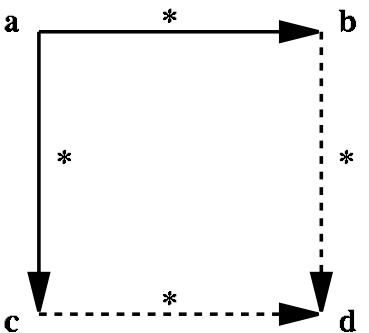
\includegraphics[scale=0.3]{img/Church-Rosser.png}
 %\captionsetup{labelformat=empty}
 \caption{丘奇-罗瑟定理的示意}
 \label{fig:Church-Rosser-confluence}
%\end{figure}
\end{wrapfigure}

更耐人寻味的是这个例子:$(\lambda x . 1)\ (D\ D)$,如果先化简$(\lambda x . 1)$,那么化简过程会中止,答案为1。反之如果先化简$(D\ D)$,则根据上面的结论,这一过程就会陷入“死循环”而无法中止。丘奇和他的学生罗瑟\footnote{罗瑟(John Barkley Rosser Sr. 1907 - 1989)是美国数学家、逻辑学家。除了丘奇-罗瑟定理外,罗瑟还和克莱尼一起还提出了克莱尼-罗瑟悖论,在数论领域,他提出了罗瑟筛法,并证明了罗瑟定理,该定理指出,第$n$个素数$p_n > n \ln n$。罗瑟在1936年还给出了一种更强的哥德尔第一不完全定理的形式,他把不可判定命题改进为:“对本命题的任何证明,都存在一个对否命题的更短证明。”}在1936年证明了一对定理,完整地回答了第二个问题。

\index{丘奇-罗瑟定理}
\begin{theorem}[丘奇-罗瑟定理一]
若$E_1 \leftrightarrow E_2$,则存在$E$,使得$E_1 \to E$且$E_2 \to E$。
\end{theorem}

也就是说,如果化简过程是可终止的,则化简结果是一致的。不同的化简方法会化简到同一结果,如图\ref{fig:Church-Rosser-confluence}所示。在此基础上,丘奇和罗瑟又证明了第二定理。为此我们先要给出“范式”(Normal form)的概念,所谓范式,又称$\beta$范式,是指不能再进行$\beta$-规约的形式。简单来讲,就是表达式中能够应用的函数都已经应用了。更严格的范式是$\beta-\eta$范式,在这样的范式中,既不能进行$\beta$-规约,也不能进行$\eta$-规约。例如$(x \mapsto x + 1)\ y$不是范式,因为它可以进行$\beta$-规约变成$y + 1$。下面是范式的递归定义。

\[
\begin{array}{rcll}
normal((\lambda x . y)\ z) & = & \textbf{false} & \text{可进一步$\beta$-规约} \\
normal(\lambda x . (f\ x)) & = & \textbf{false} & \text{可进一步$\eta$-规约} \\
normal(x\ y) & = & normal(x) \land normal(y) & \text{应用:函数和参数都是范式} \\
normal(x) & = & \textbf{true} & \text{其它情况}
\end{array}
\]

\begin{theorem}[丘奇-罗瑟定理二]
若$E_1 \to E_2$,且$E_2$为范式,则存在从$E_1$化简到$E_2$的正规顺序。
\end{theorem}

注意,这一定理要求化简过程也必须是可终止的。所谓正规顺序(normal order)就是从左向右,从外向内的化简顺序。

\section{递归的定义}

利用上一节中介绍的$\lambda$抽象,我们已经可以定义一些简单函数,但是如何定义递归函数呢?比如阶乘,它可以递归地定义为:

\[
fact = n \mapsto \textbf{if}\ n = 0\ \textbf{then}\ 1\ \textbf{else}\ n \times fact (n - 1)
\]

但这并不是一个合法的$\lambda$表达式,问题是由于$\lambda$抽象只定义了匿名函数,而我们并未定义如何给函数命名。再次观察递归的阶乘定义,它形如:

\[
fact = n \mapsto (... fact ...)
\]

我们反向使用$\beta$-规约(即$\beta$-抽象),将其变换为:

\[
fact = (f \mapsto (n \mapsto (... f ...)))\ fact
\]

进一步可以抽象为

\be
fact = H\ fact
\label{eq:H-fact}
\ee

其中

\[
H = f \mapsto (n \mapsto (... f ...))
\]

\index{不动点}
注意到,经过这样的变换,我们得到的$H$不再是递归的,它是一个普通的$\lambda$表达式。观察式(\ref{eq:H-fact}),它表示了递归。在形式上它是一个数学方程,让我们联想起“微分方程”的概念。例如解微分方程$y' = sin(x)$得到$y = a - cos(x)$。如果我们能将方程$F = H\ F$解出,就能完整地定义阶乘了。进一步观察,我们发现这个方程的含义是,将$H$应用到$F$上,得到的结果仍然是$F$。这一概念在数学上叫做“不动点”。我们称$F$是$H$的不动点。再举一个不动点的例子:$\lambda$表达式$x \mapsto x \times x$的不动点是0和1,这是因为$(x \mapsto x \times x)\ 0 = 0$且$(x \mapsto x \times x)\ 1 = 1$。

\subsection{Y组合子}
\index{Y组合子}
我们希望找到$H$的不动点,显然$H$的不动点只依赖于$H$本身。为此,我们引入一个函数$Y$,它接受一个函数,然后返回这个函数的不动点。$Y$的行为表现如下:

\be
Y\ H = H\ (Y\ H)
\label{eq:Y-H}
\ee

为此$Y$被称为“不动点组合子”(fixpoint combinator)。使用$Y$,我们就得到了方程(\ref{eq:H-fact})的解:

\be
fact = Y\ H
\label{eq:fact-in-Y}
\ee

这样得到的$fact$是一个无递归的定义。我们可以这样验证这个解:

\[
\begin{array}{rcll}
fact & = & Y\ H & \text{式(\ref{eq:fact-in-Y})} \\
     & = & H\ (Y\ H) & \text{式(\ref{eq:Y-H})} \\
     & = & H\ fact & \text{式(\ref{eq:fact-in-Y})反向}
\end{array}
\]

$Y$的强大之处在于它可以表达所有的递归函数。但是现在的$Y$仍然是个黑盒子,我们需要用$\lambda$抽象来真正实现它。下面就是$Y$的实现:

\be
Y = \lambda h . (\lambda x . h\ (x\ x))\ (\lambda x . h\ (x\ x))
\ee

写成箭头形式为:

\[
Y = h \mapsto (x \mapsto h\ (x\ x)) (x \mapsto h\ (x\ x))
\]

我们打开了潘多拉的魔盒,现在来验证一下这个$Y$的$\lambda$抽象是否表现得符合我们的预期:$Y\ H = H\ (Y\ H)$。

\begin{proof}
\[
\begin{array}{rcll}
Y\ H & = & (h \mapsto (x \mapsto h\ (x\ x)) (x \mapsto h\ (x\ x)))\ H & \text{$Y$的定义} \\
     & \xleftrightarrow{\beta} & (x \mapsto H\ (x\ x))\ (x \mapsto H\ (x\ x)) & \text{$\beta$-规约,用$H$代换$h$} \\
     & \xleftrightarrow{\alpha} & (y \mapsto H\ (y\ y))\ (x \mapsto H\ (x\ x)) & \text{对前半部分用$\alpha$-变换} \\
     & \xleftrightarrow{\beta} & H\ ((x \mapsto H\ (x\ x))\ (x \mapsto H\ (x\ x))) & \text{$\beta$-规约,$y$被后半部代换} \\
     & \xleftrightarrow{\beta} & H\ (h \mapsto (x \mapsto h\ (x\ x))\ (x \mapsto h\ (x\ x))\ H) & \text{$\beta$-抽象,$H$抽出为参数} \\
     & = & H\ (Y\ H) & \text{代入$Y$的定义}
\end{array}
\]
\end{proof}

最终,使用$Y$,我们可以如下实现阶乘的定义:

\[
Y\ (f \mapsto (n \mapsto \textbf{if}\ n = 0\ \textbf{then}\ 1\ \textbf{else}\ n \times f\ (n - 1)))
\]

用$\lambda$-抽象来定义$Y$的数学意义远大于其实现的意义。在真实的环境中,通常$Y$被内置实现为函数,可以直接将$Y\ H$转化为$H\ (Y\ H)$。

\section{$\lambda$演算的意义}

$\lambda$演算的意义在于,它用一组简单的规则对复杂的计算过程进行了定义。将欧几里得算法用$\lambda$演算表示出来,再利用$\beta$规约进行计算。这样的实现可能比较复杂,但确实可行。它不仅可以表达欧几里得算法,而且适用于所有的可计算函数。图灵后来证明了$\lambda$演算与图灵机的等价性。$\lambda$演算的一大优势在于它仅仅使用了传统的数学概念——函数。因而在十九世纪30年代,$\lambda$演算被用来对数学进行形式化。然而在1935年,克莱尼-罗瑟悖论证明了最初的$\lambda$形式系统在逻辑上是不一致的。1936年,丘奇将$\lambda$演算模型中和纯计算有关的部分分离出来,称为的无类型$\lambda$演算。1940年时,丘奇又提出了一个弱化计算,但是逻辑自洽的形式系统,被称之为简单类型$\lambda$演算。

我们展示了如何用$\lambda$演算定义基本的四则运算、逻辑运算、定义和应用普通函数以及递归函数。最后,我们给出如何用$\lambda$演算定义复合数据结构。我们用此前定义的$cons$、$head$、$tail$作为例子。以下是它们的$\lambda$抽象定义:

\[
\begin{array}{rcl}
cons & = & (\lambda a . \lambda b . \lambda f . f\ a\ b) \\
head & = & (\lambda c . c\ (\lambda a . \lambda b . a)) \\
tail & = & (\lambda c . c\ (\lambda a . \lambda b . b))
\end{array}
\]

写成箭头形式为:

\[
\begin{array}{rcl}
cons & = & a \mapsto b \mapsto f \mapsto f\ a\ b \\
head & = & c \mapsto c\ (a \mapsto b \mapsto a) \\
tail & = & c \mapsto c\ (a \mapsto b \mapsto b)
\end{array}
\]

我们来验证一下$head\ (cons\ p\ q) = p$这一关系。

\[
\begin{array}{rcl}
head\ (cons\ p\ q) & = & (c \mapsto c\ (a \mapsto b \mapsto a))\ (cons\ p\ q) \\
                   & \xrightarrow{\beta} & (cons\ p\ q)\ (a \mapsto b \mapsto a) \\
                   & = & ((a \mapsto b \mapsto f \mapsto f\ a\ b)\ p\ q)\ (a \mapsto b \mapsto a) \\
                   & \xrightarrow{\beta} & ((b \mapsto f \mapsto f\ p\ b)\ q)\ (a \mapsto b \mapsto a) \\
                   & \xrightarrow{\beta} & (f \mapsto f \mapsto f\ p\ q)\ (a \mapsto b \mapsto a) \\
                   & \xrightarrow{\beta} & (a \mapsto b \mapsto a)\ p\ q \\
                   & \xrightarrow{\beta} & (b \mapsto p)\ q \\
                   & \xrightarrow{\beta} & p
\end{array}
\]

这说明,理论上复合数据结构不必一定要内置实现,而可以用$\lambda$定义。本章练习中还展示了如何用$\lambda$演算基于皮亚诺公理系统定义自然数、布尔值及逻辑运算。

\begin{Exercise}
\Question{使用$\lambda$变换规则验证$tail\ (cons\ p\ q) = q$。}
\Question{可以仅仅使用$\lambda$演算来定义自然数。下面是丘奇数的定义:
\[
\begin{array}{r@{\quad:\quad}l}
0 & \lambda f . \lambda x . x \\
1 & \lambda f . \lambda x . f\ x \\
2 & \lambda f . \lambda x . f\ (f\ x) \\
3 & \lambda f . \lambda x . f\ (f\ (f\ x)) \\
  & ...
\end{array}
\]
请利用第一章介绍的内容,定义丘奇数的加法和乘法。
}
\Question{以下是丘奇布尔值的定义,以及逻辑运算的一种实现:
\[
\begin{array}{r@{\quad:\quad}l}
\textbf{true} & \lambda x . \lambda y . x \\
\textbf{false} & \lambda x . \lambda y . y \\
\textbf{and} & \lambda p . \lambda q . p\ q\ p \\
\textbf{or} & \lambda p . \lambda q . p\ p\ q \\
\textbf{not} & \lambda p . p\ \textbf{false}\ \textbf{true}
\end{array}
\]
其中\textbf{false}的定义和丘奇数0的定义本质上是相同的。试用$\lambda$变换证明:\textbf{and}\ \textbf{true}\ \textbf{false} = \textbf{false};你能给出if...then...else...语句的$\lambda$定义么?
}
\end{Exercise}

\section{更多的递归结构}

至此,我们已经将递归函数和递归数据结构建立在完整的数学基础上。利用这些工具,我们可以继续定义一些较复杂的数据结构。例如下面的二叉树。

\lstset{frame=none}
\begin{lstlisting}
data Tree A = nil | node (Tree A, A, Tree A)
\end{lstlisting}

这个递归定义说,一棵元素类型为A的二叉树或者为空,或者是一个分支节点。节点包含三部分:两棵元素类型为A的子树和一个类型为A的元素。习惯上我们称这两棵子树为左子树和右子树。A是类型参数,例如自然数。$node(nil, 0, node(nil, 1, nil))$表示了一棵元素为自然数的二叉树。下面我们为二叉树定义抽象的叠加操作$foldt$。

\be
\begin{array}{l}
foldt(f, g, c, nil) = c \\
foldt(f, g, c, node(l, x, r)) = g(foldt(f, g, c, l), f(x), foldt(f, g, c, r))
\end{array}
\ee

如果函数$f$将类型为A的自变量映射为类型为B的值,我们将其类型记为$f : A \to B$。克里化的函数$foldt(f, g, c)$的类型为$foldt(f, g, c) : Tree\ A \to B$,其中$c$的类型为$B$,而函数$g$的类型为$g : (B \times B \times B) \to B$,写成克里化的形式为$g : B \to B \to B \to B$。使用抽象的叠加函数$foldt$我们可以定义针对二叉树的逐一映射$mapt$:

\be
mapt(f) = foldt(f, node, nil)
\ee

通过叠加操作,还可以定义函数来统计一棵二叉树中的元素个数:

\be
sizet = foldt(one, sum, 0)
\ee

其中$one(x) = 1$,是一个常数函数,它对任何变量都返回1。$sum$是一个三元的累加函数:$sum(a, b, c) = a + b + c$。

在此基础上,复合使用第一章定义的列表,我们还可以从二叉树扩展到多叉树,下面是一个多叉树的定义:

\begin{lstlisting}
data MTree A = nil | node (A, List (MTree A))
\end{lstlisting}

一棵元素类型为A的多叉树或者为空,或者为一个复合节点。复合节点包括一个类型为A的元素,和若干子树。所有子树用一个多叉树的列表来表示。定义多叉树的抽象叠加操作需要相互递归调用列表的叠加操作。

\be
\begin{array}{l}
foldm(f, g, c, nil) = c \\
foldm(f, g, c, node(x, ts)) = foldr(g(f(x), c), h, ts) \\
h(t, z) = foldm(f, g, z, t)
\end{array}
\ee

\begin{Exercise}
\Question{不用抽象的叠加操作$foldt$,通过递归定义二叉树的逐一映射$mapt$;}
\Question{定义一个函数$depth$,计算一棵二叉树的最大深度;}
\Question{有人认为,二叉树的抽象叠加操作$foldt$应该这样定义:
\[
\begin{array}{l}
foldt(f, g, c, nil) = c \\
foldt(f, g, c, node(l, x, r)) = foldt(f, g, g(foldt(f, g, c, l), f(x)), r)
\end{array}
\]
也就是说,$g : (B \times B) \to B$是一个类似于加法这样的二元函数。能否利用这个$foldt$定义逐一映射$mapt$?}
\Question{排序二叉树(又称二叉搜索树)是一种特殊的二叉树,如果二叉树的元素类型A是可比较的,并且对任何非空节点$node(l, k, r)$都满足:左子树$l$中的任何元素都小于$k$,右子树$r$中的任何元素都大于$k$。定义二叉树的插入函数$insert(x, t) : (A \times Tree\ A) \to Tree\ A$}
\Question{为多叉树定义逐一映射。能否利用多叉树的叠加操作来定义?如果不能,应当怎样修改叠加操作?}
\end{Exercise}

\section{递归的形式与结构}

递归不仅存在于古老的欧几里得算法和现代计算机系统中,它迷人的形式和结构还出现在各种人类文明艺术中。图\ref{fig:Ceramic-Tile-Tessellations-Marrakech}的平面镶嵌中,可以看到多重不同的递归形式。

%\begin{wrapfigure}{R}{0.3\textwidth}
\begin{figure}[htbp]
 \centering
 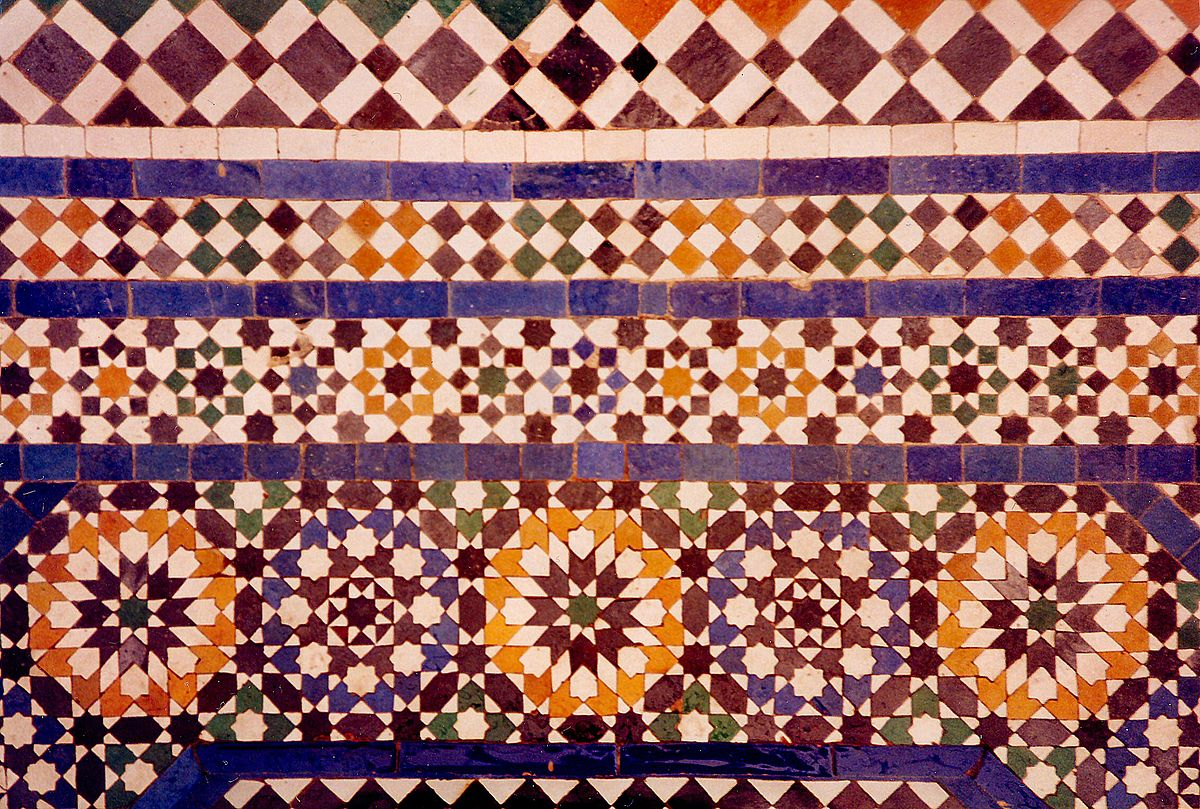
\includegraphics[scale=1]{img/Marrakech.jpg}
 %\captionsetup{labelformat=empty}
 \caption{马拉喀什(摩洛哥城市)的瓷砖图案}
 \label{fig:Ceramic-Tile-Tessellations-Marrakech}
\end{figure}
%\end{wrapfigure}

我们可以看到瓷砖中的多边形图案中递归地含有更小的多边形嵌套。通过不同颜色的瓷砖,这种递归展现出几何形式的美。这些图案还在更大的范围组成条纹形式,而各个条纹内部都是不同的递归图形。图\ref{fig:flower}左边展示的是文艺复兴时期艺术大师达$\cdot$芬奇手稿中的递归图样。在圆周上使用相同的半径,依次可作出六个相互交织的圆,从而构成一个六瓣的花样图案。而在更大的范围上,又递归地构成了同样形式的图案。右侧图案是中国民间手工编织的蝈蝈笼子,他们展示了类似的递归图样。笼子的网眼是六边形的,而笼子的整体形状从轴向看去也是六边形的。

%\begin{wrapfigure}{R}{0.3\textwidth}
\begin{figure}[htbp]
 \centering
 \subcaptionbox{达芬奇绘制的递归图案手稿}[0.3\linewidth]{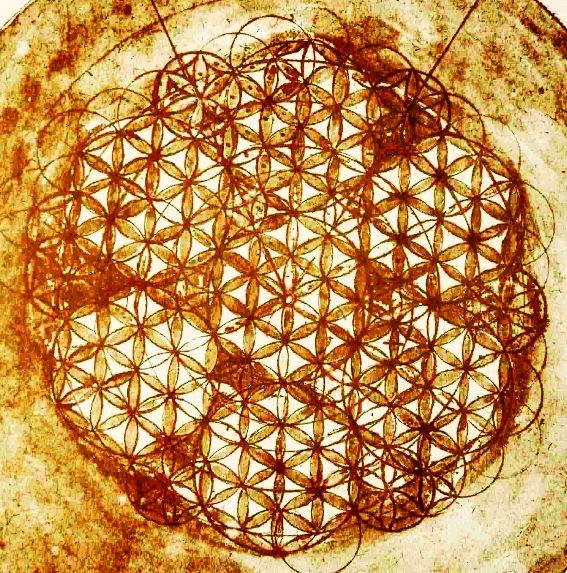
\includegraphics[scale=0.20]{img/ldv_flower.jpg}} \quad
 \subcaptionbox{手工编织的蝈蝈笼子}[0.5\linewidth]{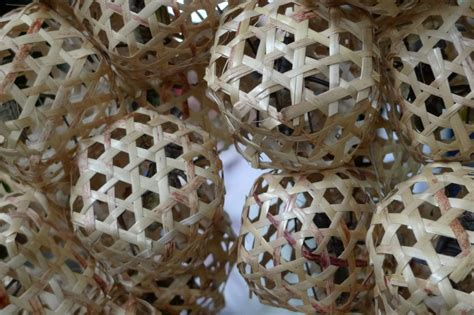
\includegraphics[scale=0.36]{img/cage.jpg}}
 %\captionsetup{labelformat=empty}
 \caption{艺术和生活物品中的递归形式}
 \label{fig:flower}
\end{figure}
%\end{wrapfigure}

递归不仅出现在美术作品中,还出现在更加抽象的艺术形式中,例如音乐。复调音乐中的卡农(Canon)和赋格(Fugue)都是这方面的代表。卡农的所有声部虽然都模仿一个声部,但不同高度的声部依一定间隔进入,造成一种此起彼伏,连绵不断的效果。每一个声部都地归地展示主题但却含有各种变化,比如音调的升高或降低、逆行重叠、速度变快(减值)或变慢(增值)、旋律倒影等等。

%\begin{wrapfigure}{L}{0.45\textwidth}
\begin{figure}[htbp]
 \centering
 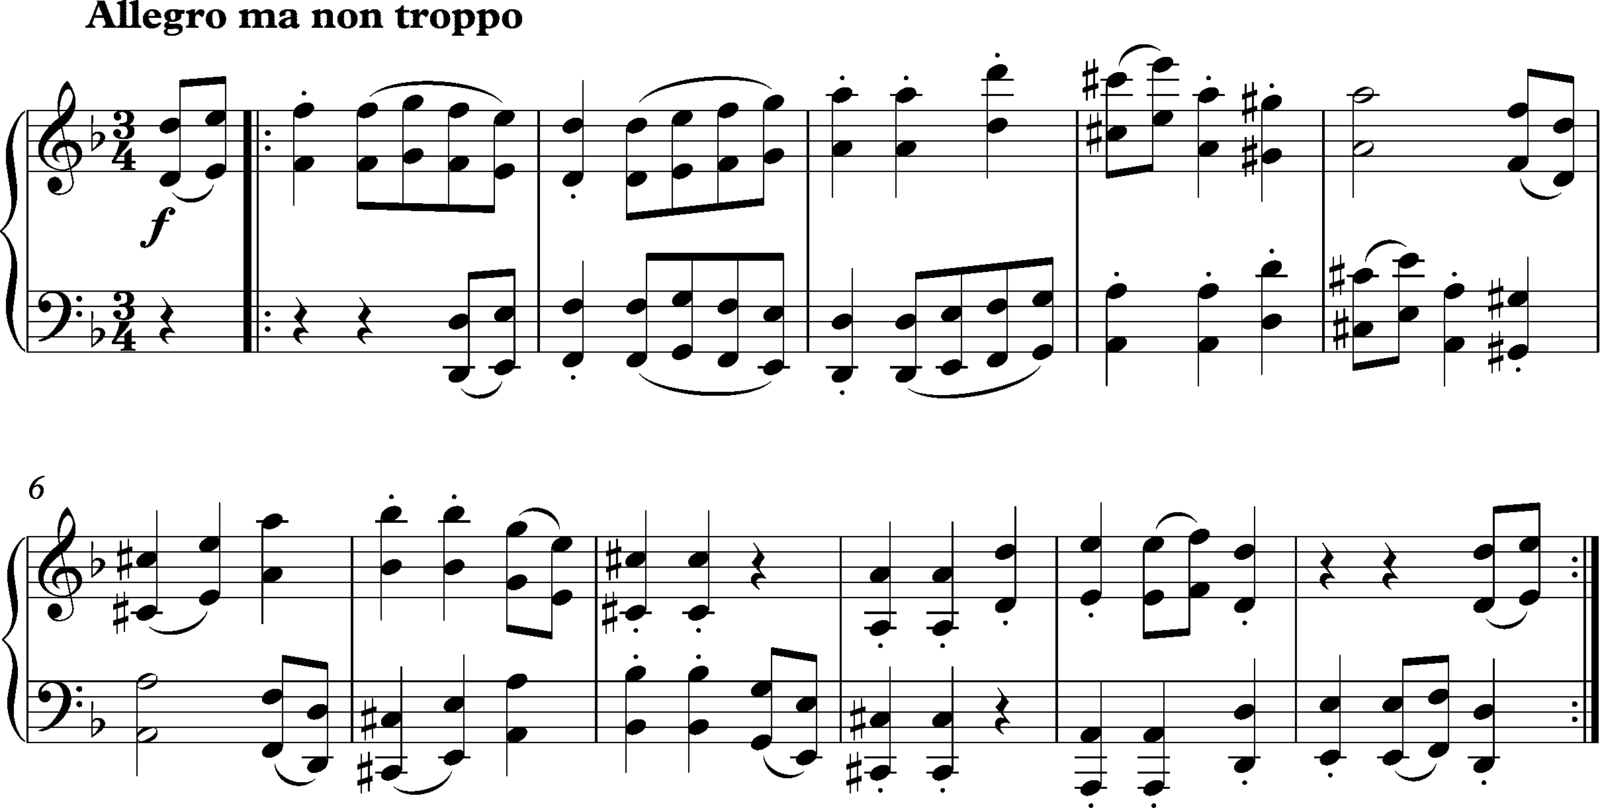
\includegraphics[scale=0.8]{img/Haydn-OP-76.png}
 %\captionsetup{labelformat=empty}
 \caption{海顿D小调弦乐四重奏小步舞曲,作品76第2}
 \label{fig:Haydn-OP-76}
\end{figure}
%\end{wrapfigure}

%\begin{wrapfigure}{L}{0.45\textwidth}
\begin{figure}[htbp]
 \centering
 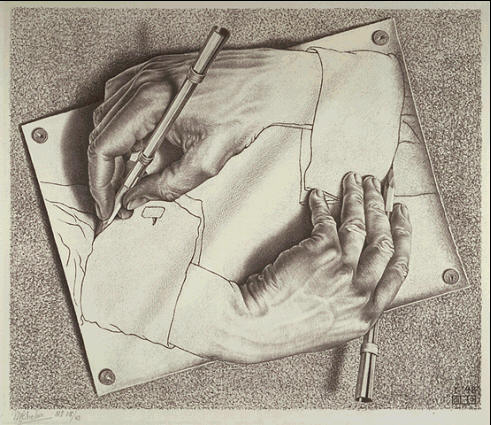
\includegraphics[scale=0.6]{img/Drawing-Hands-1948.jpg}
 %\captionsetup{labelformat=empty}
 \caption{艾舍尔的作品《画手》,1948年}
 \label{fig:Drawing-Hands}
\end{figure}
%\end{wrapfigure}

赋格通常建立在一个主题上,以不同的声部、不同的调子、偶尔也用不同的速度或上下颠倒或从后往前地进行演奏。然而,赋格的概念远不如卡农那么严格,因而允许有更多的情感或艺术的表现。赋格的识别标志的是它的开始方式:单独的一个声部唱出它的主题,唱完后,第二个声部或移高五度或降低四度进入。与此同时,第一个声部继续唱“对应主题”,也叫第二主题,用来在节奏、和声、及旋律方面与主题形成对比。每个声部依次唱出主题,常常是另一个声部伴唱对应主题,其它的声部所起的作用随作曲家的想象而定。当所有的声部都“到齐”了,就不再有什么规则了。当然,还是有一些标准的手法,但它没有严格到只能够按照某个公式去创作赋格。 《音乐的奉献》 中的两首赋格曲就是杰出例子,它们绝不可能“照公式创造出来”。这两首曲子都具有远比赋格的性质更为深刻的东西\cite{GEB}。

这些都是有限递归的例子。图\ref{fig:Drawing-Hands}是荷兰艺术大师艾舍尔在1948年创作的《画手》,两只手递归地在描绘着对方。《画手》是无穷递归的典型例子。画中上方的手正在用一支笔描绘着下方的手,而下方的手也在地归地描绘着上方的手。这组相互递归的嵌套一层一层,无穷无尽。

无穷递归的一个数学与艺术完美结合的例子是“分形”(fractal)。例如著名的分形图案“科克雪花”(Kock snowflake)曲线可以通过这样的无穷递归规则来产生:对图形中的每个线段,均分为三段,以第二段为底向上方作出一个等边三角形,然后再把这个底擦掉。图\ref{fig:fractal}中展示了三重递归后从一个正三角形得到的科克雪花。另一个著名的递归分形图案是谢尔平斯基三角形(Sierpinski),它的生成规则是对图形中的每个三角形,分别取三边的中点,连成一个内部的小三角形,然后“挖掉这个内部的小三角形”。下图展示了递归四次后的谢尔平斯基三角形。

%\begin{wrapfigure}{R}{0.3\textwidth}
\begin{figure}[htbp]
 \centering
 \subcaptionbox{科克雪花的递归生成规则}[0.4\linewidth]{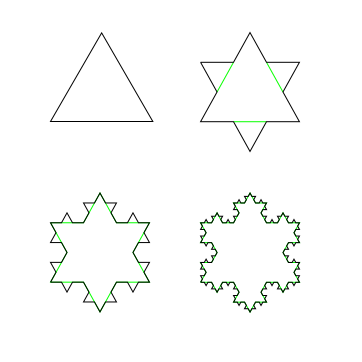
\includegraphics[scale=0.25]{img/KochFlake.png}}
 \subcaptionbox{谢尔平斯基三角形}[0.4\linewidth]{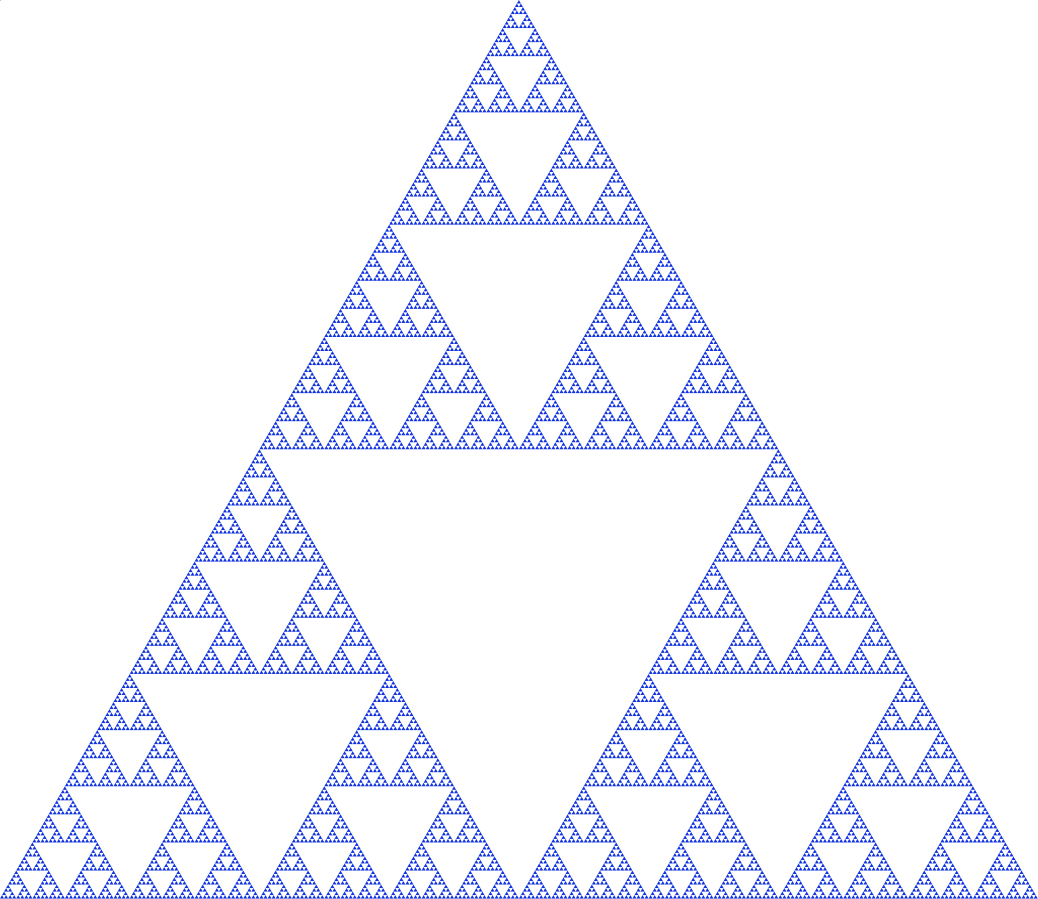
\includegraphics[scale=0.1]{img/Sierpinski-triangle.png}}
 %\captionsetup{labelformat=empty}
 \caption{递归产生的分形图案}
 \label{fig:fractal}
\end{figure}
%\end{wrapfigure}

最后让我们以两张分形图案来结束本章,其中一张是人类思维产生的分形——茱莉亚集(Julia);另一张是自然界产生的分形。

\begin{figure}[htbp]
 \centering
 \subcaptionbox{茱莉亚集分形}[0.45\linewidth]{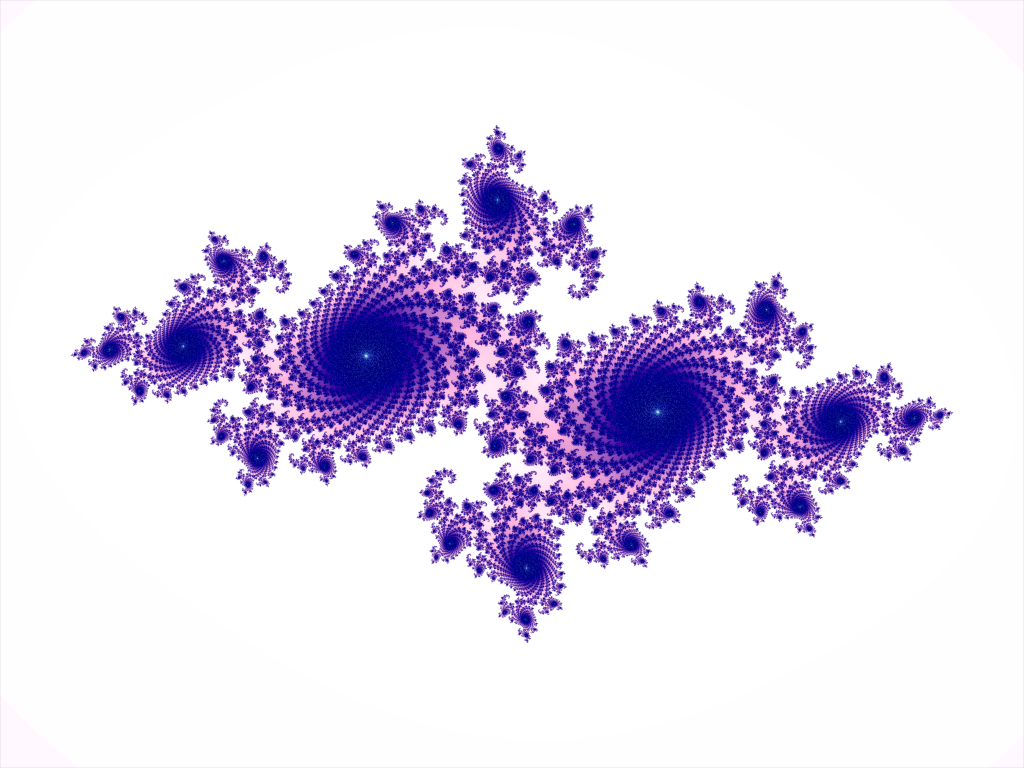
\includegraphics[scale=0.18]{img/Julia_set.png}}
 \subcaptionbox{西兰花中的分形}[0.45\linewidth]{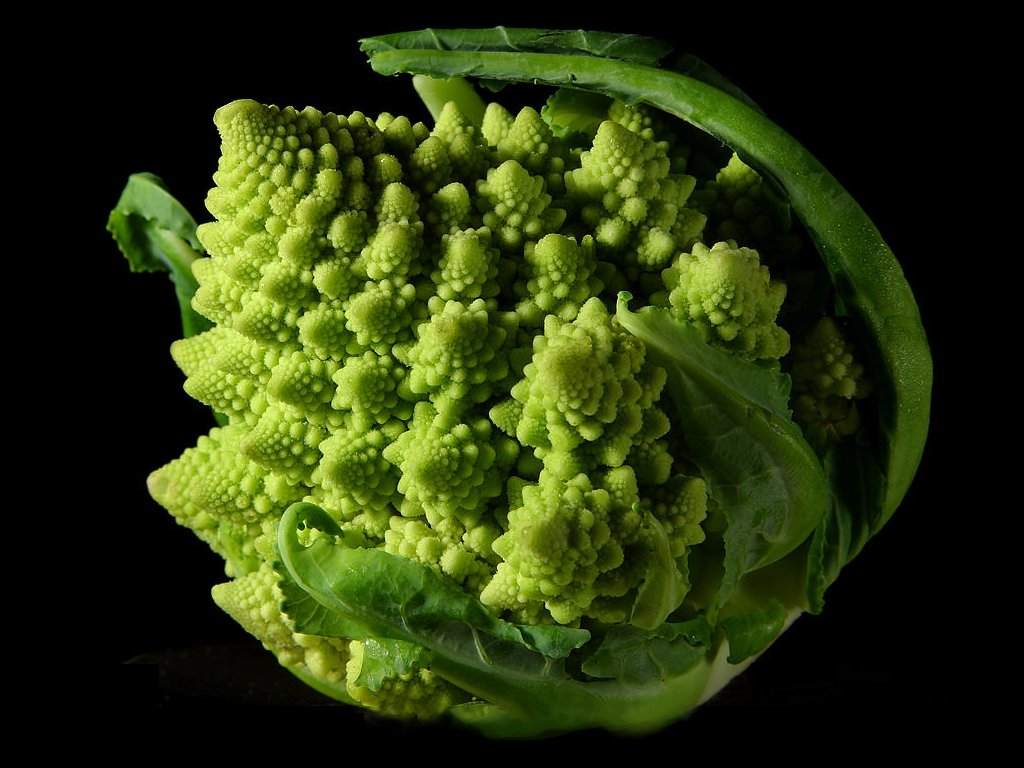
\includegraphics[scale=0.2]{img/Broccoli.jpg}}
 %\captionsetup{labelformat=empty}
 \caption{人类思维和自然界产生的分形}
 \label{fig:more-fractal}
\end{figure}

\section{扩展阅读}

韩雪涛的《数学悖论与三次数学危机》\cite{HanXueTao16}对古希腊数学的成就有生动的介绍。欧几里得的《几何原本》中译本\cite{Elements}是永远的经典。斯捷潘诺夫和罗斯的《数学与泛型编程》\cite{StepanovRose15}中有欧几里得算法算法的多种实现。随着各大主流编程环境引入lambda演算,这方面的介绍材料很多。佩顿琼斯的《函数式编程语言的实现》\cite{SPJ1987}讲解全面并且深入浅出。侯世达先生的《集异璧》\cite{GEB}中有大量关于递归的介绍和奇思妙想,曾获得普利策大奖。中译本秉着文化同构的精神进行了非凡的再创作。

\section{附录:倒水趣题完整程序}

求得两个瓶子倒水的次数后,就可以生成一系列倒水的步骤,将这些步骤像表(\ref{tab:designed-jugs-ops})一样输出。

\lstset{frame=single}
\begin{lstlisting}
-- Populate the steps
water a b c = if x > 0 then pour a x b y
              else map swap $ pour b y a x
  where
    (x, y) = jars a b c

-- Pour from a to b, fill a for x times, and empty b for y times.
pour a x b y = steps x y [(0, 0)]
  where
    steps 0 0 ps = reverse ps
    steps x y ps@((a', b'):_)
      | a' == 0 = steps (x - 1) y ((a, b'):ps)  -- fill a
      | b' == b = steps x (y + 1) ((a', 0):ps)  -- empty b
      | otherwise = steps x y ((max (a' + b' - b) 0,
                                min (a' + b') b):ps) -- a to b
\end{lstlisting}

运行这一程序,输入\texttt{water 9 4 6}就可以得到最佳的倒水步骤:

\begin{verbatim}
[(0,0),(9,0),(5,4),(5,0),(1,4),(1,0),(0,1),(9,1),(6,4),(6,0)]
\end{verbatim}

\ifx\wholebook\relax \else
\begin{thebibliography}{99}

\bibitem{HanXueTao16}
韩雪涛 ``数学悖论与三次数学危机''. 人民邮电出版社. 2016, ISBN: 9787115430434

\bibitem{MKlein1972}
[美] 莫里斯$\cdot$克莱因 张理京等译 ``古今数学思想,第一册''. 上海科学技术出版社. 2014, ISBN: 9787547817179

\bibitem{StepanovRose15}
[美] 亚历山大 A$\cdot$斯捷潘诺夫,丹尼尔 E$\cdot$罗斯著,爱飞翔译. ``数学与泛型编程:高效编程的奥秘''. 机械工业出版社. 2017, ISBN: 9787111576587

\bibitem{Elements}
[古希腊] 欧几里得 著,兰纪正 朱恩宽 译,梁宗巨 张毓新 徐伯谦 校订 ``几何原本''. 译林出版社. 2014, ISBN: 9787544750066

\bibitem{HanXueTao2009}
韩雪涛 ``好的数学——“下金蛋”的数学问题''. 湖南科学技术出版社. 2009, ISBN: 9787535756725

\bibitem{Bezout-Identity}
Wikipedia ``贝祖等式'' \url{https://en.wikipedia.org/wiki/Bézout's_identity}

\bibitem{LiuXinyu2017}
刘新宇 ``算法新解'' 人民邮电出版社. 2017, ISBN: 9787115440358

\bibitem{wiki-Turing}
Wikipedia ``艾伦$\cdot$图灵'' \url{https://en.wikipedia.org/wiki/Alan_Turing}

\bibitem{Dowek2011}
[法] 吉尔$\cdot$多维克 著,劳佳 译 ``计算进化史:改变数学的命运''. 人民邮电出版社. 2017, ISBN: 9787115447579

\bibitem{SPJ1987}
Simon L. Peyton Jones. ``The implementation of functional programming language''. Prentice Hall. 1987, ISBN: 013453333X

\bibitem{GEB}
[美]候世达 ``哥德尔、埃舍尔、巴赫——集异壁之大成''. 商务印书馆 1996. ISBN: 978-7-100-01323-9

\end{thebibliography}

\expandafter\enddocument
%\end{document}

\fi
